\documentclass[a4paper,11pt]{article}
\usepackage[utf8]{inputenc}
\usepackage[top=0.8cm, bottom=0.8cm, left=1cm, right=1cm]{geometry}
\usepackage{amsmath}
\usepackage{graphicx}
\usepackage{caption}
\usepackage[hidelinks]{hyperref}

% Configurazione didascalie compatte per preservare l'altezza pagina
\captionsetup[figure]{font=small, labelfont=bf, skip=2pt}
\setlength{\parindent}{0pt}
\title{\textbf{Analisi delle Prestazioni di Modelli Centralizzati ILP per il Task Routing al variare della Deadline}}
\author{Claudio Bagini 2045337}
\date{\today}

\begin{document}

\maketitle

Il presente documento sintetizza i risultati della campagna sperimentale condotta sull'orchestratore centralizzato ILP, valutando l'esplorazione esaustiva dei parametri di batching ($BS \in \{1, \dots, 20\}$, $BT \in [0.0, 2.0]\text{ s}$) e di instradamento topologico. I grafici sono strutturati per metrica di riferimento --- tasso di successo (\textit{Success Rate}), distribuzione delle cause di rigetto (\textit{Rejection Causes}) e scomposizione del tempo di risposta (\textit{Stacked Response Time}) --- e confrontano sistematicamente le prestazioni al variare del carico di traffico ($\lambda \in [2, 10]\text{ req/s}$), della tolleranza temporale ($\Delta D \in \{10\%, 20\%, 30\%\}$) e dell'obiettivo di allocazione adottato (\textit{Energy Mapping} rispetto a \textit{Time Mapping}).
\vspace{1em}


% ==============================================================================
% 1. SUCCESS RATE
% ==============================================================================

% --- Success Rate: Energy Mapping (DL 10, 20, 30) ---
\begin{center}
    \textbf{\Large Task Success Rate --- Energy Mapping ($w_{lat}=0, w_{en}=1$)}
\end{center}
\vspace{-0.3em}

\makebox[\textwidth][c]{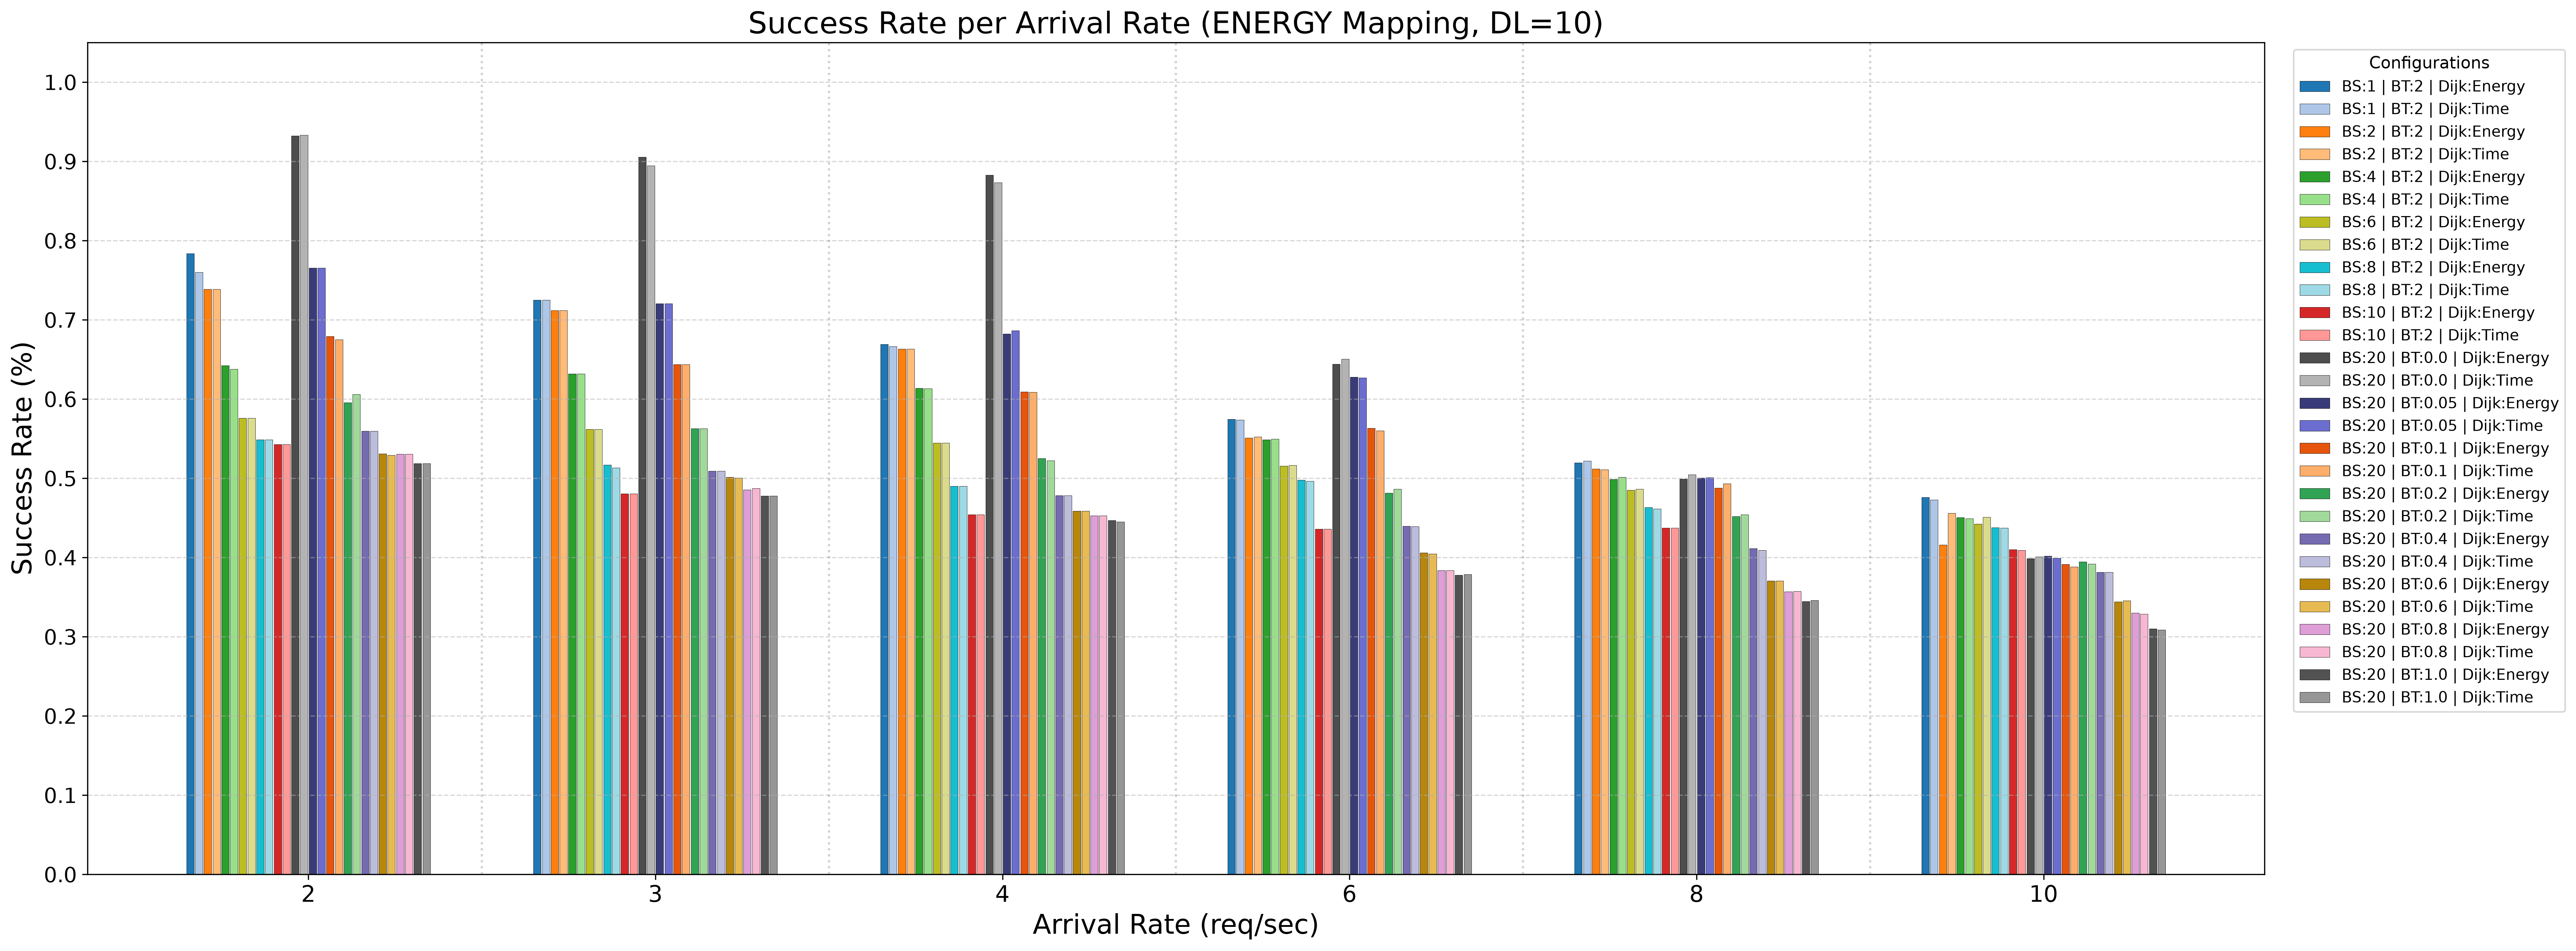
\includegraphics[width=\paperwidth]{01_Success_Rate_energy_mapping_dl_10.png}}
\captionof{figure}{Success Rate across arrival rates ($\Delta D = 10\%$).}
\vspace{0.4em}

\makebox[\textwidth][c]{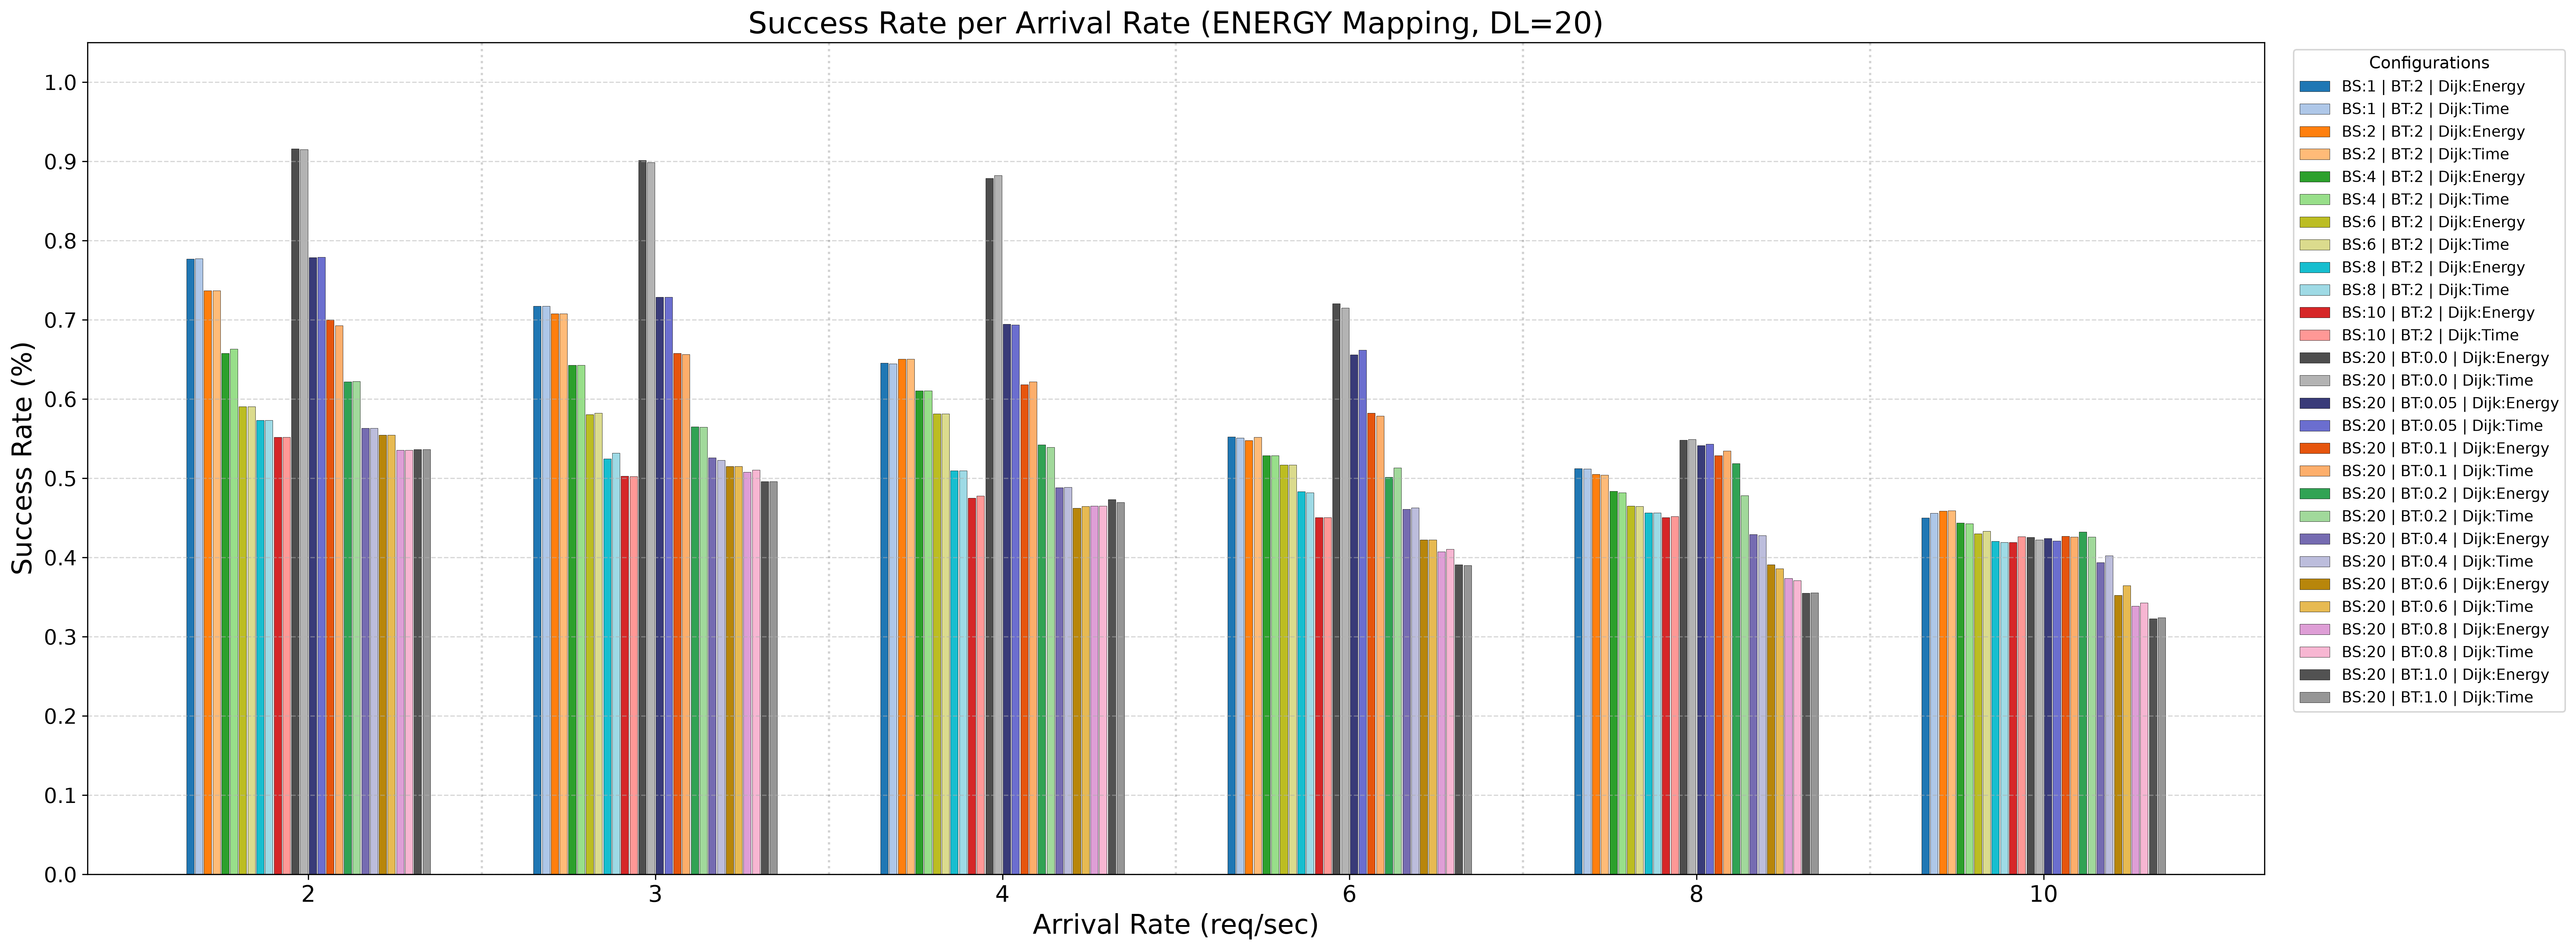
\includegraphics[width=\paperwidth]{01_Success_Rate_energy_mapping_dl_20.png}}
\captionof{figure}{Success Rate across arrival rates ($\Delta D = 20\%$).}
\vspace{0.4em}

\makebox[\textwidth][c]{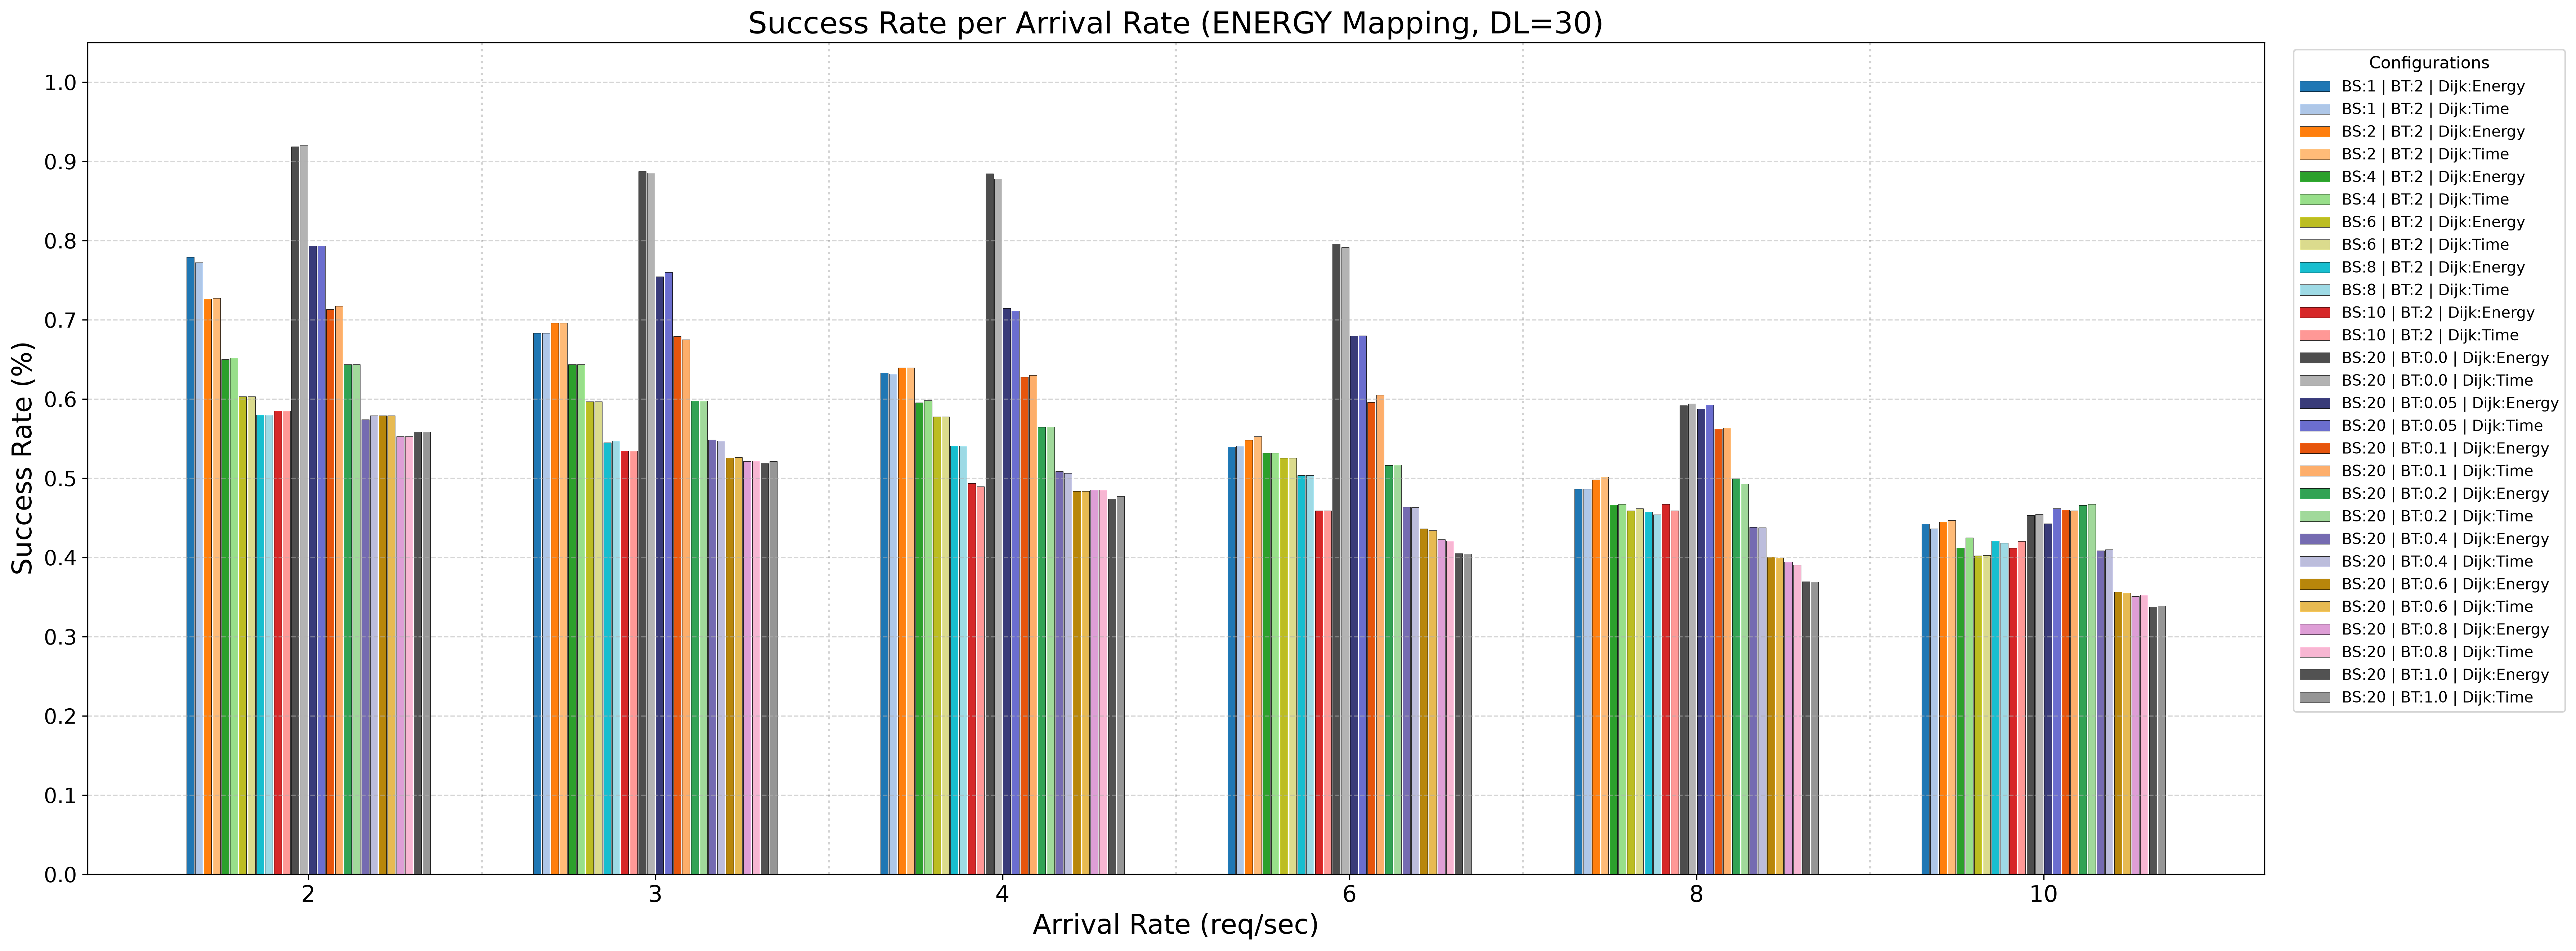
\includegraphics[width=\paperwidth]{01_Success_Rate_energy_mapping_dl_30.png}}
\captionof{figure}{Success Rate across arrival rates ($\Delta D = 30\%$).}



% --- Success Rate: Time Mapping (DL 10, 20, 30) ---
\begin{center}
    \textbf{\Large Task Success Rate --- Time Mapping ($w_{lat}=1, w_{en}=0$)}
\end{center}
\vspace{-0.3em}

\makebox[\textwidth][c]{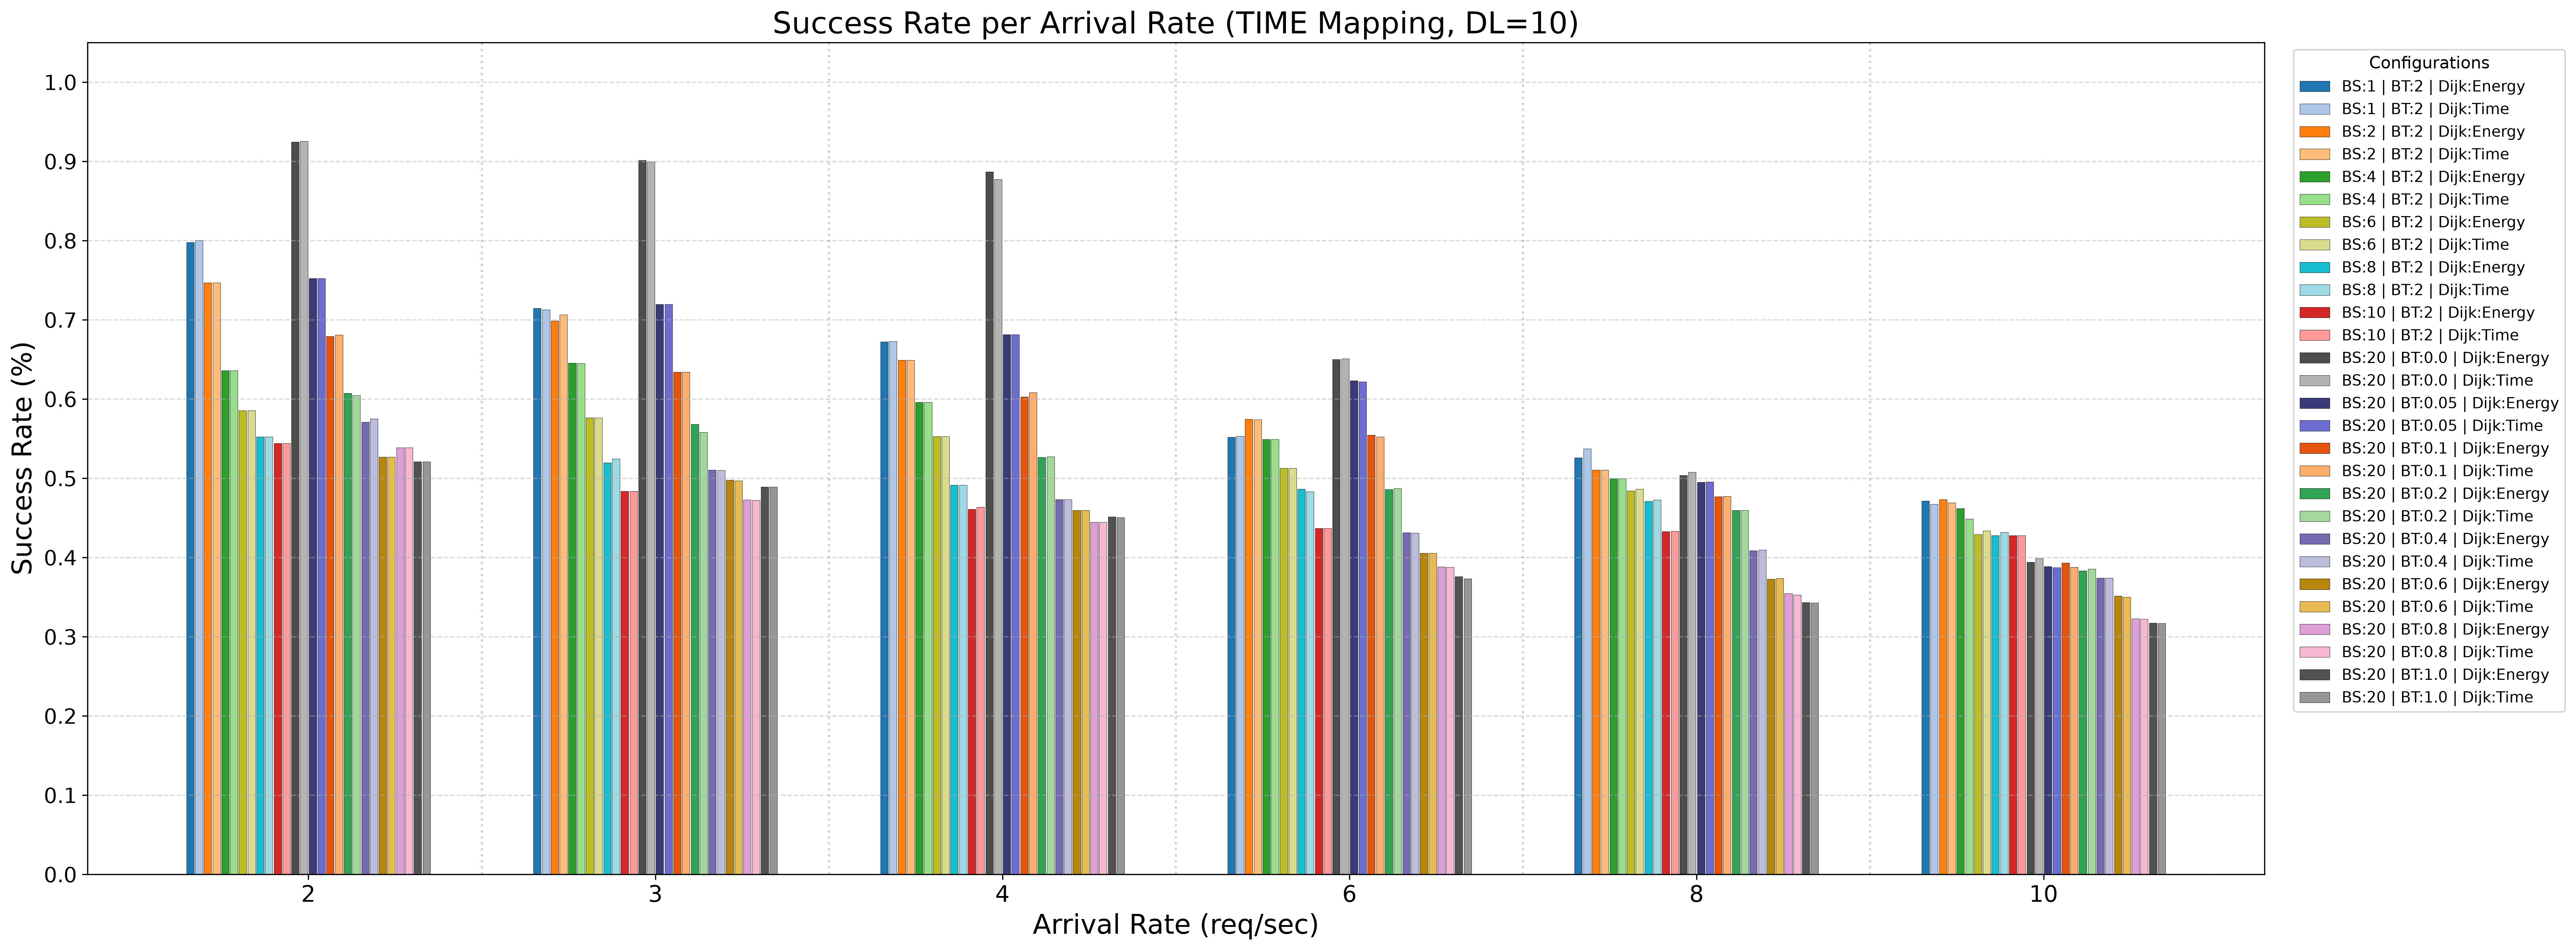
\includegraphics[width=\paperwidth]{01_Success_Rate_time_mapping_dl_10.png}}
\captionof{figure}{Success Rate across arrival rates ($\Delta D = 10\%$).}
\vspace{0.4em}

\makebox[\textwidth][c]{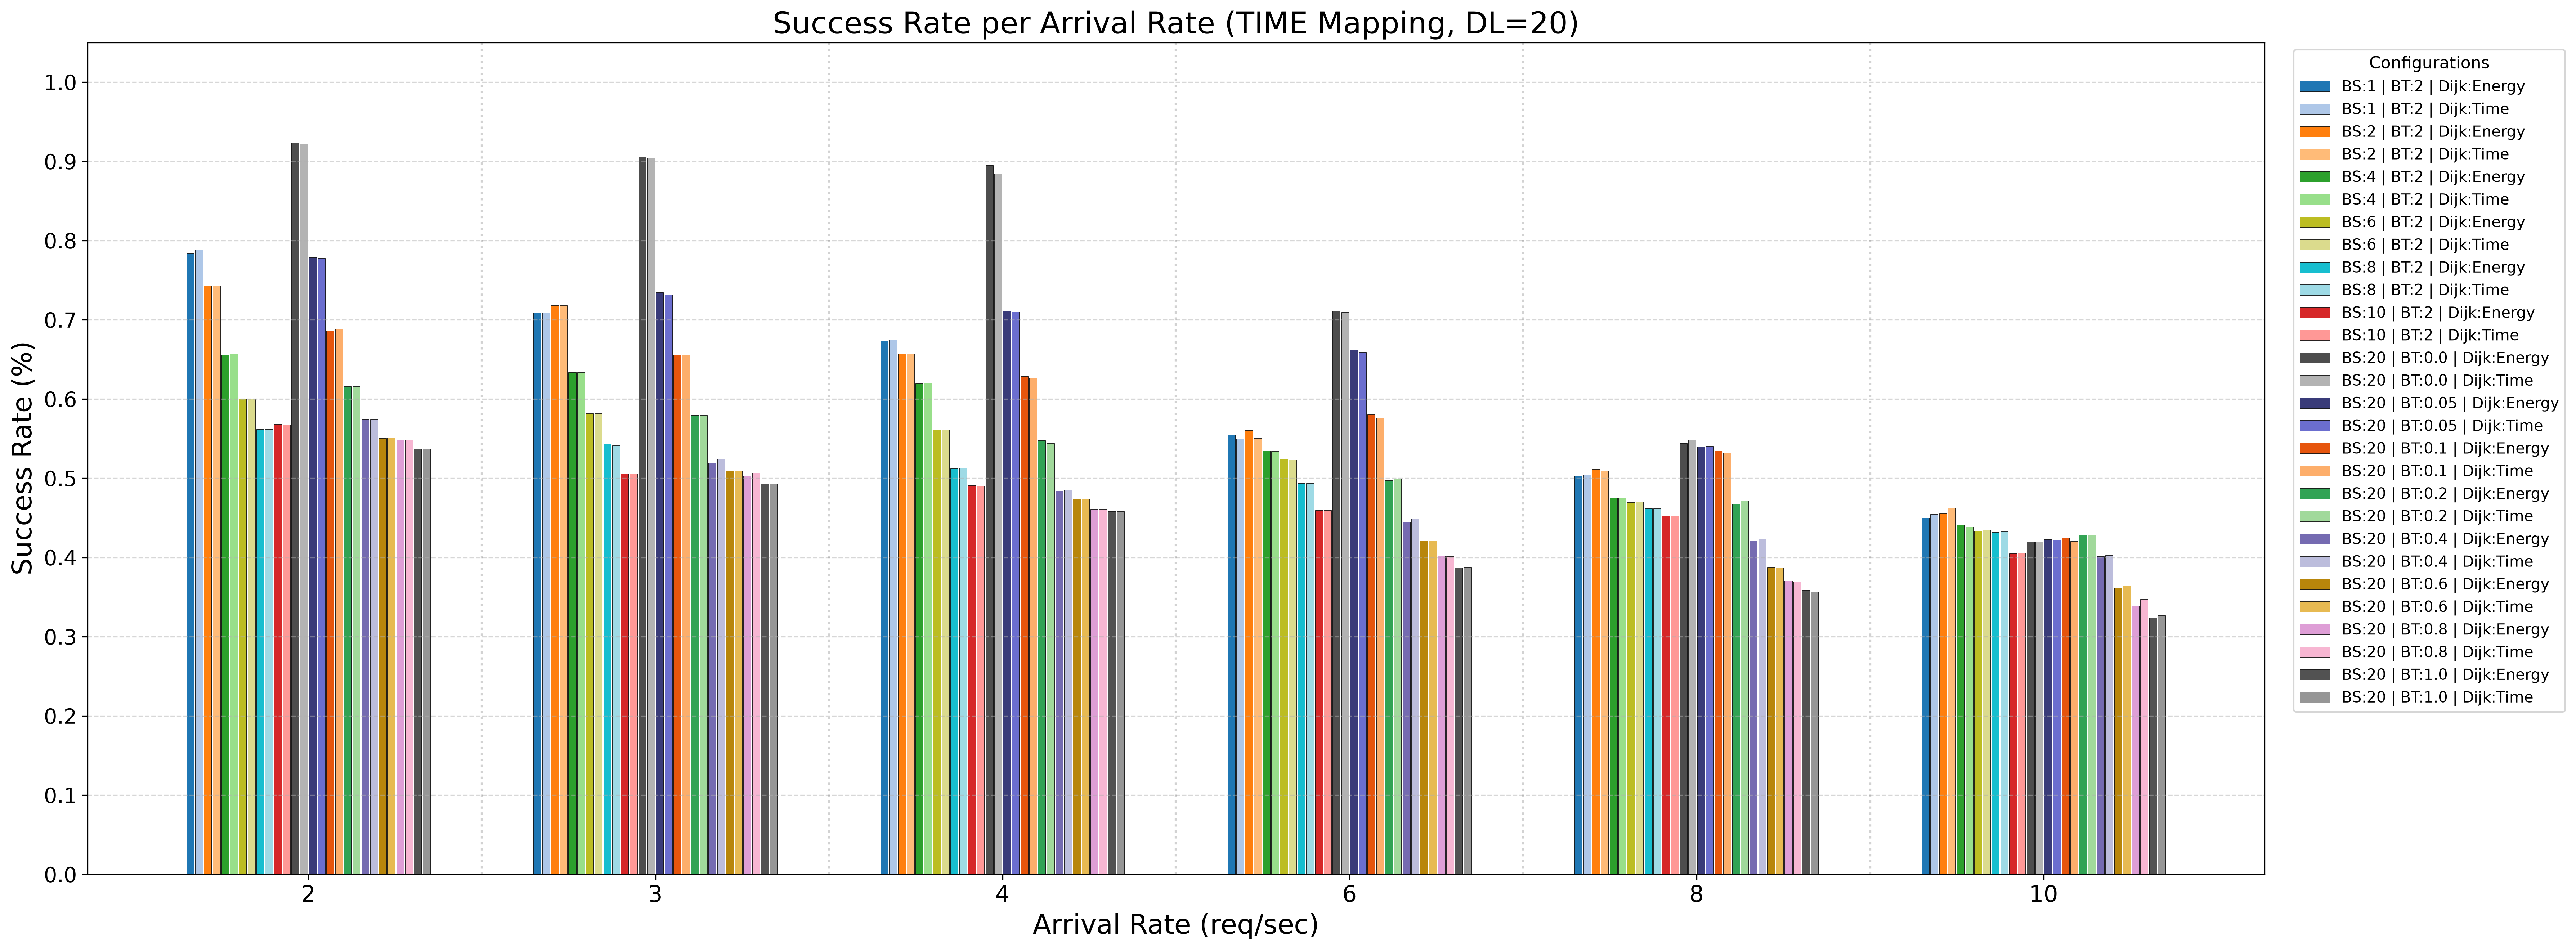
\includegraphics[width=\paperwidth]{01_Success_Rate_time_mapping_dl_20.png}}
\captionof{figure}{Success Rate across arrival rates ($\Delta D = 20\%$).}
\vspace{0.4em}

\makebox[\textwidth][c]{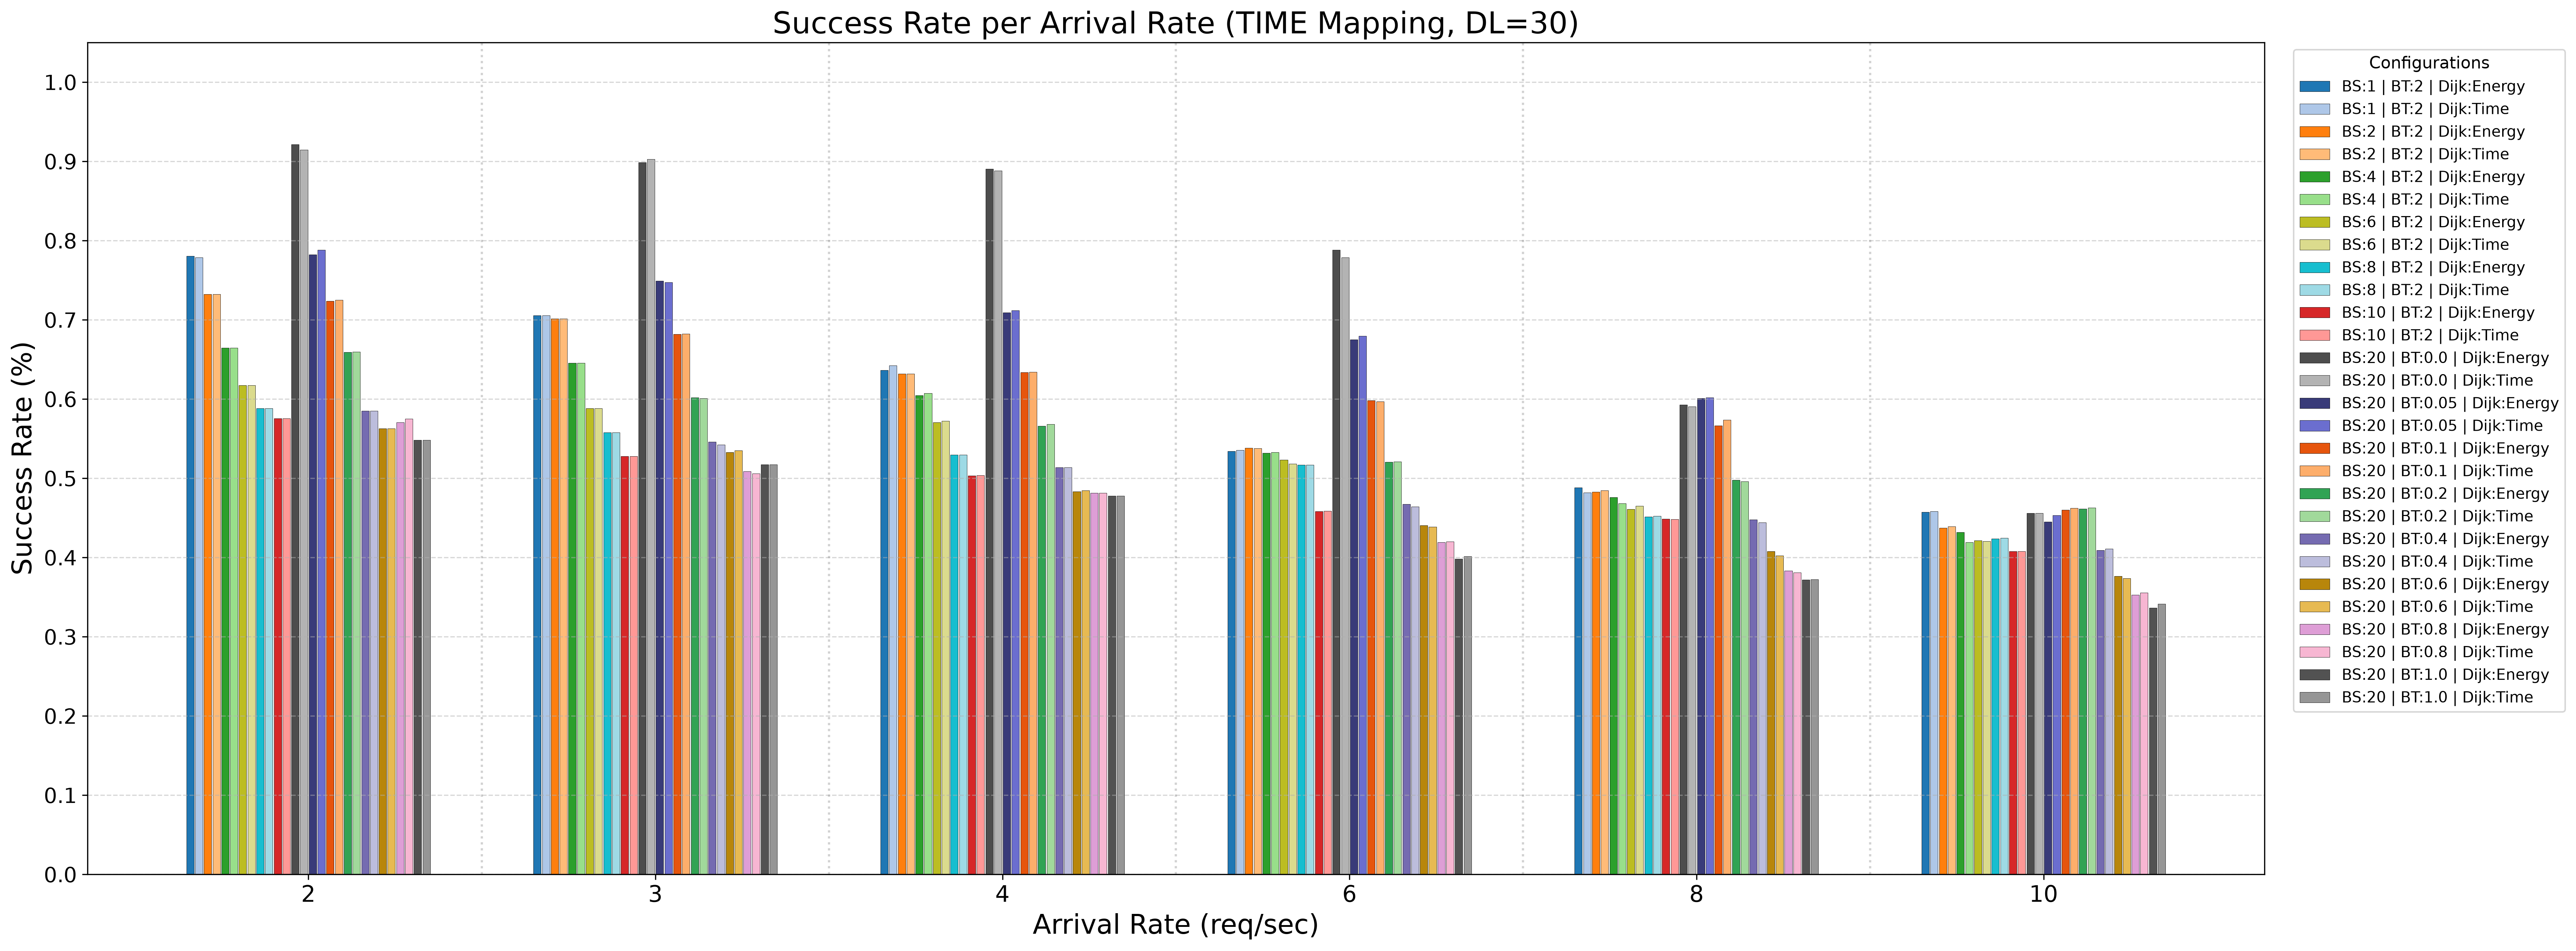
\includegraphics[width=\paperwidth]{01_Success_Rate_time_mapping_dl_30.png}}
\captionof{figure}{Success Rate across arrival rates ($\Delta D = 30\%$).}

L'analisi del tasso di successo evidenzia come il parametro determinante non sia l'obiettivo di mapping, bensì la gestione del batching: la configurazione $\text{BS}=20$ con $\text{BT}=0.0\text{ s}$ (in particolare con Dijkstra Energy) registra le prestazioni più elevate, superando il 90\% di completamento a basso carico. All'aumentare dell'arrival rate ($\lambda \to 10\text{ req/s}$), tutte le configurazioni subiscono un degrado prestazionale; tuttavia, timeout di aggregazione elevati ($\text{BT} \ge 0.4\text{ s}$) o batch ampi con attesa prolungata ($\text{BS}=10, \text{BT}=2\text{ s}$) penalizzano drasticamente il sistema già a carichi moderati, mentre il rilassamento della deadline ($\Delta D$) produce incrementi marginali.
\vspace{0.8em}

\clearpage


% ==============================================================================
% 2. REJECTION CAUSES
% ==============================================================================

% --- Rejection Causes: Energy Mapping (DL 10, 20, 30) ---
\begin{center}
    \textbf{\Large Failure Causes Distribution --- Energy Mapping ($w_{lat}=0, w_{en}=1$)}
\end{center}
\vspace{-0.3em}

\makebox[\textwidth][c]{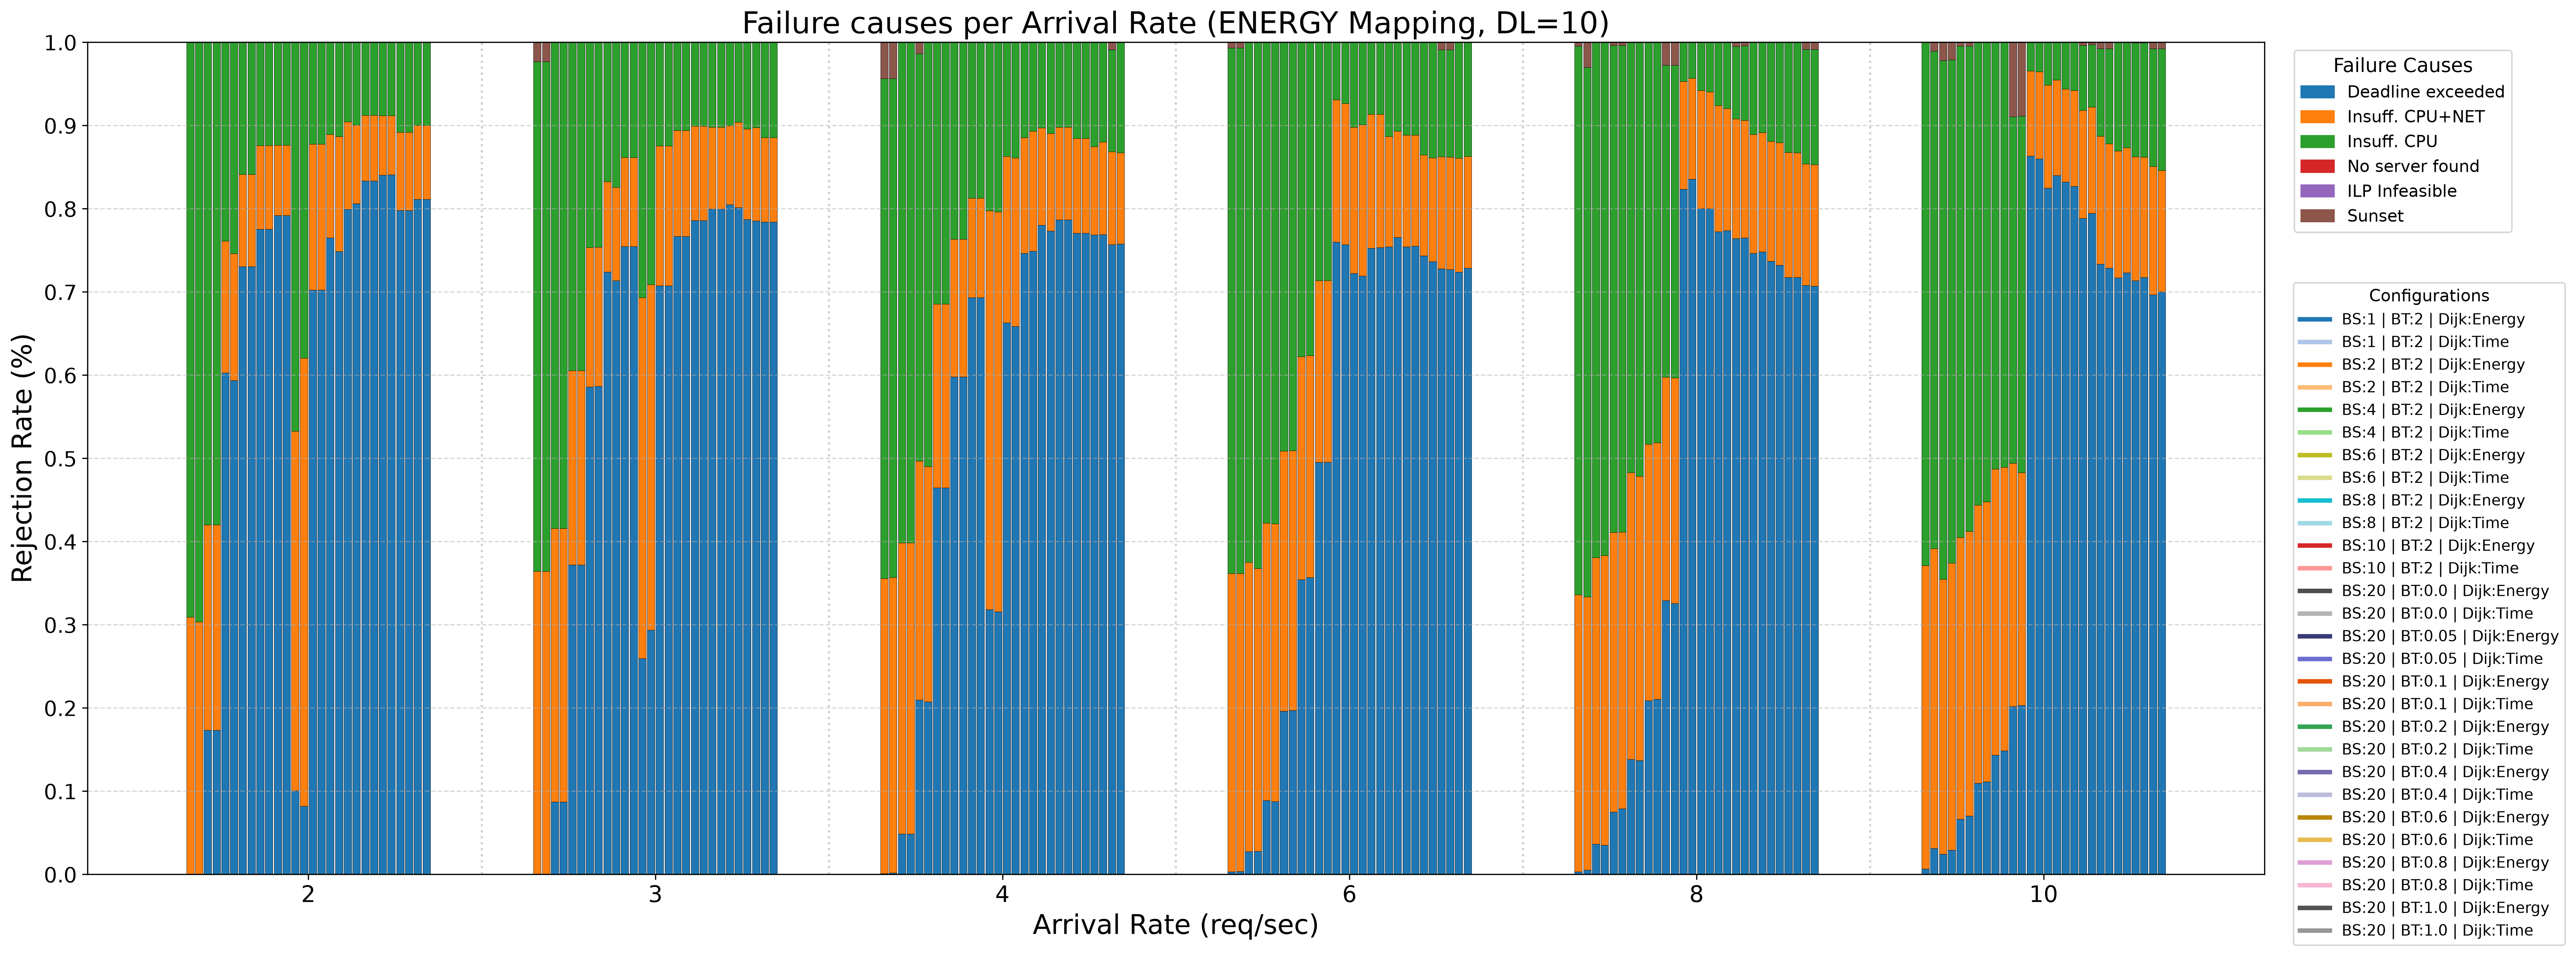
\includegraphics[width=\paperwidth]{02_Failure_Causes_energy_mapping_dl_10.png}}
\captionof{figure}{Failure Causes breakdown across arrival rates ($\Delta D = 10\%$).}
\vspace{0.4em}

\makebox[\textwidth][c]{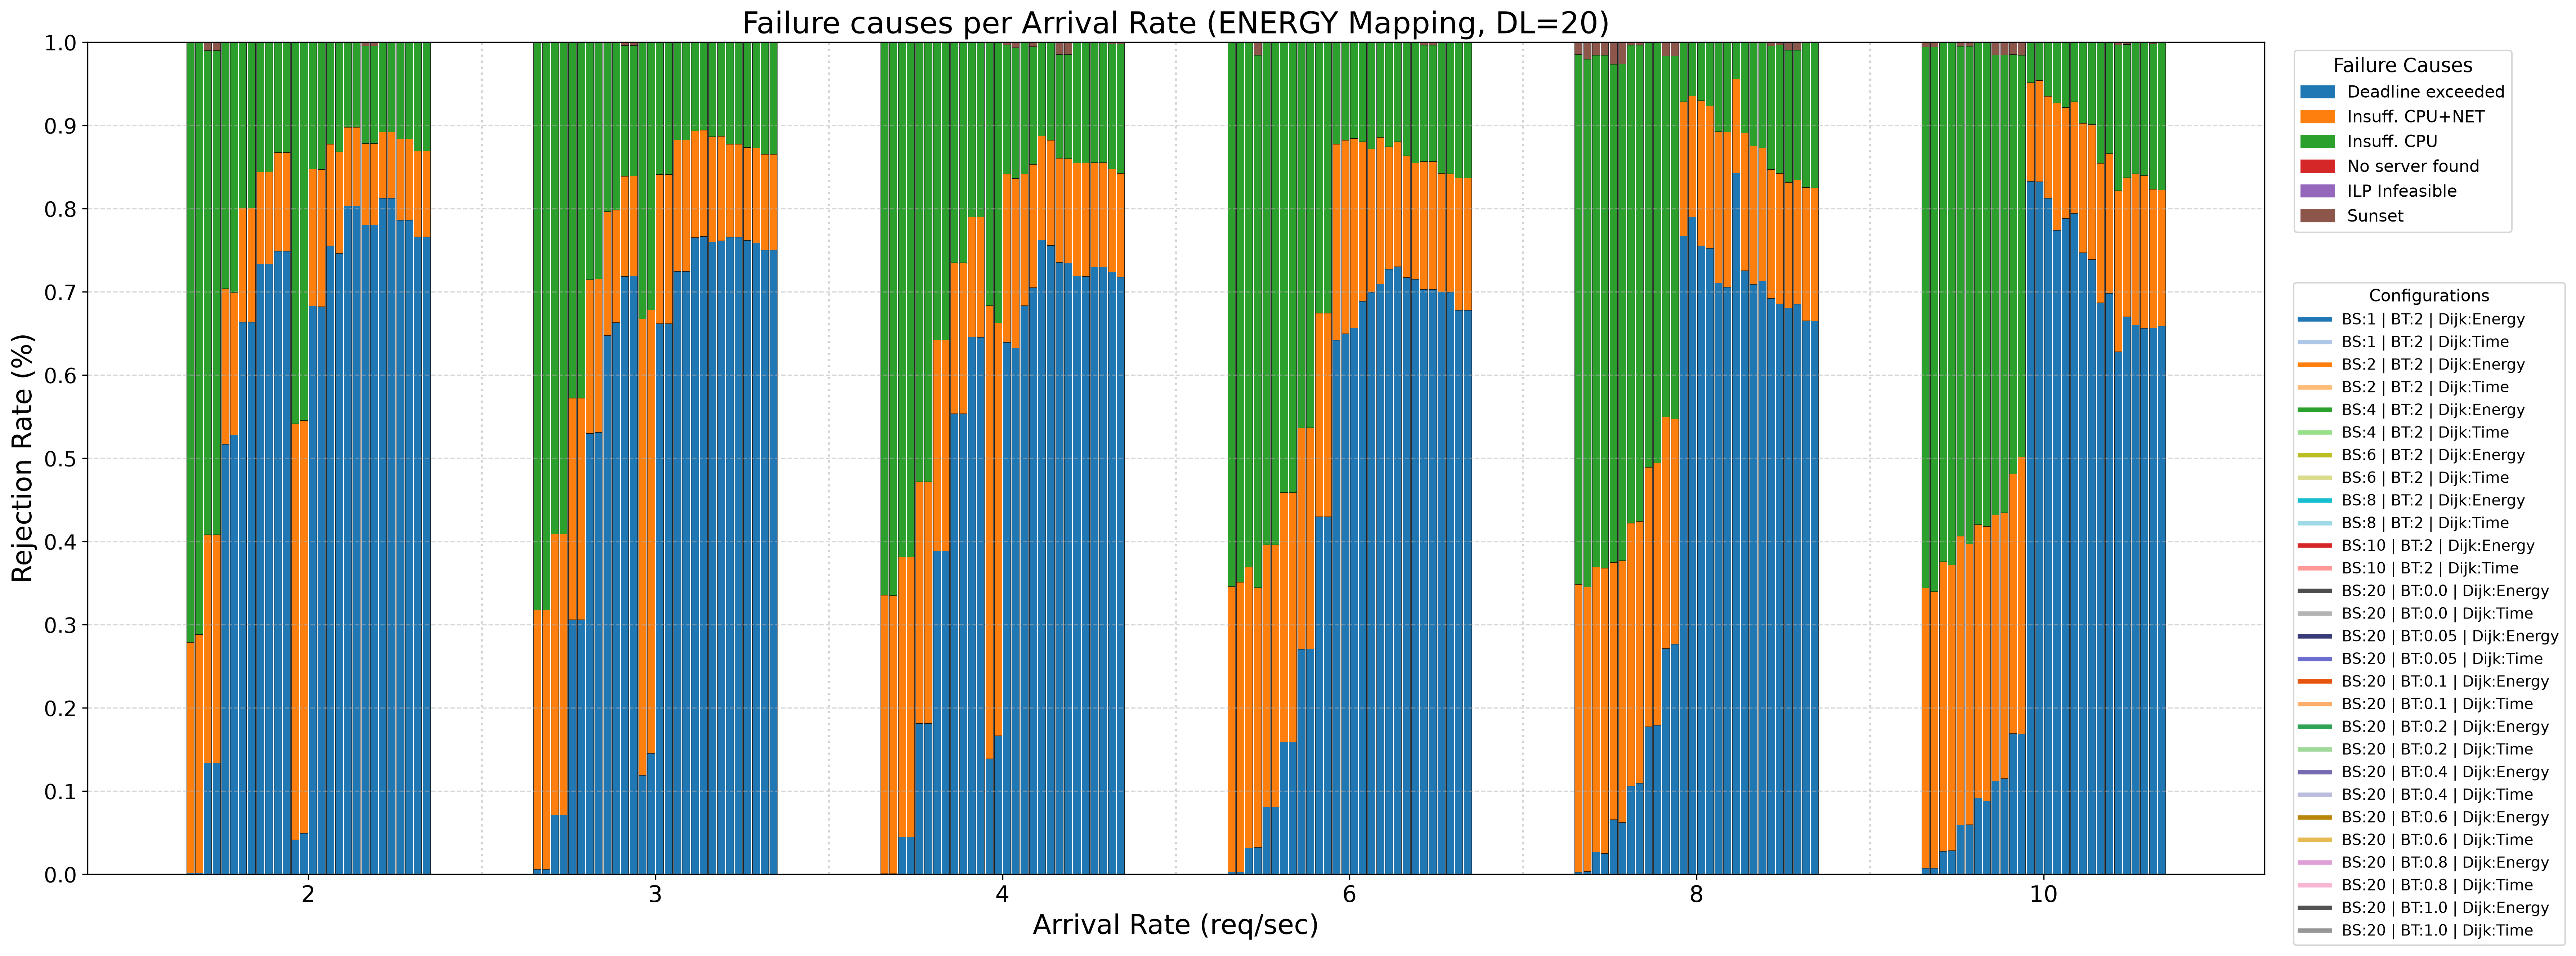
\includegraphics[width=\paperwidth]{02_Failure_Causes_energy_mapping_dl_20.png}}
\captionof{figure}{Failure Causes breakdown across arrival rates ($\Delta D = 20\%$).}
\vspace{0.4em}

\makebox[\textwidth][c]{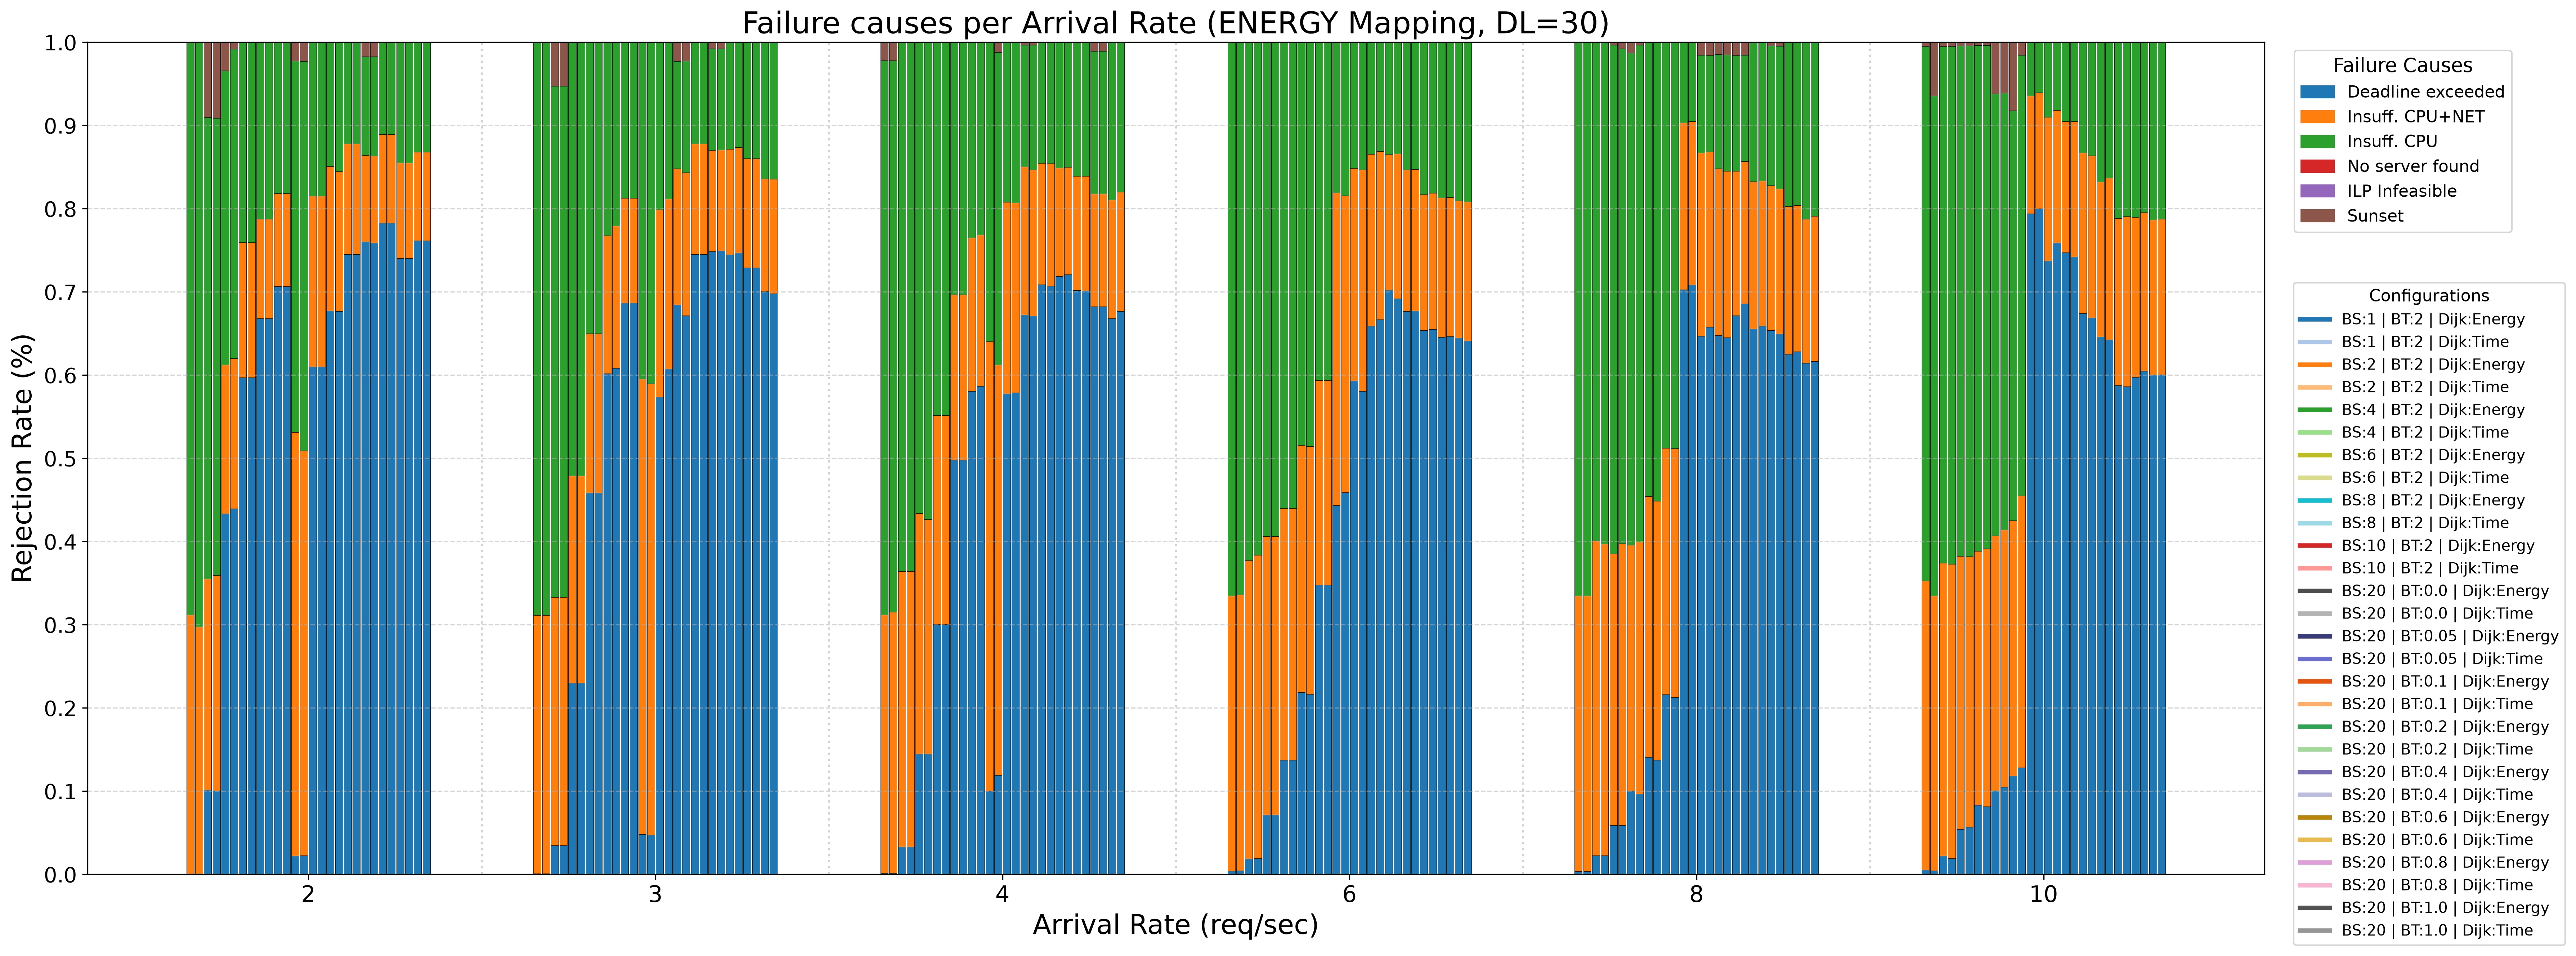
\includegraphics[width=\paperwidth]{02_Failure_Causes_energy_mapping_dl_30.png}}
\captionof{figure}{Failure Causes breakdown across arrival rates ($\Delta D = 30\%$).}



% --- Rejection Causes: Time Mapping (DL 10, 20, 30) ---
\begin{center}
    \textbf{\Large Failure Causes Distribution --- Time Mapping ($w_{lat}=1, w_{en}=0$)}
\end{center}
\vspace{-0.3em}

\makebox[\textwidth][c]{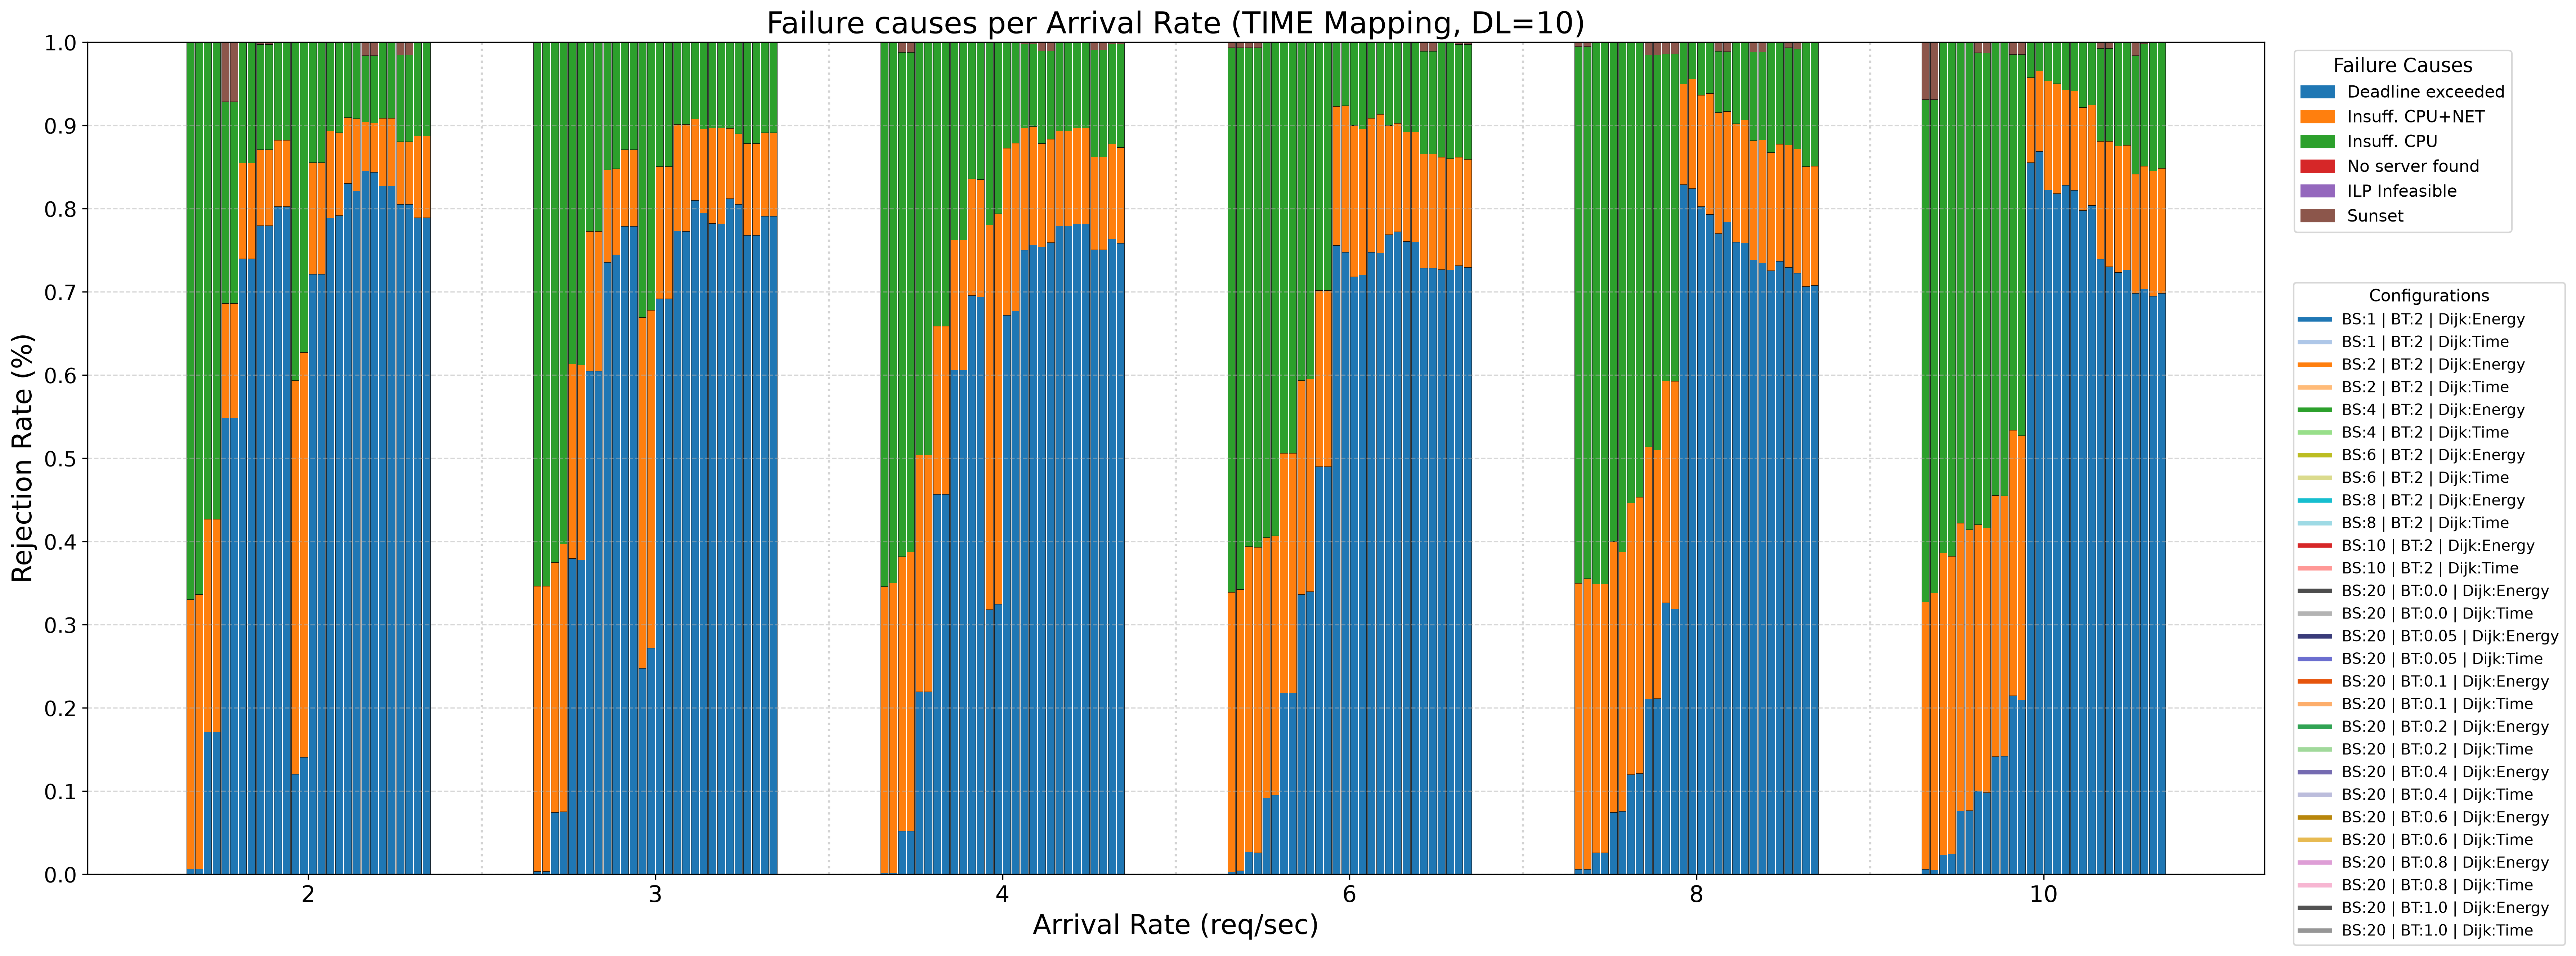
\includegraphics[width=\paperwidth]{02_Failure_Causes_time_mapping_dl_10.png}}
\captionof{figure}{Failure Causes breakdown across arrival rates ($\Delta D = 10\%$).}
\vspace{0.4em}

\makebox[\textwidth][c]{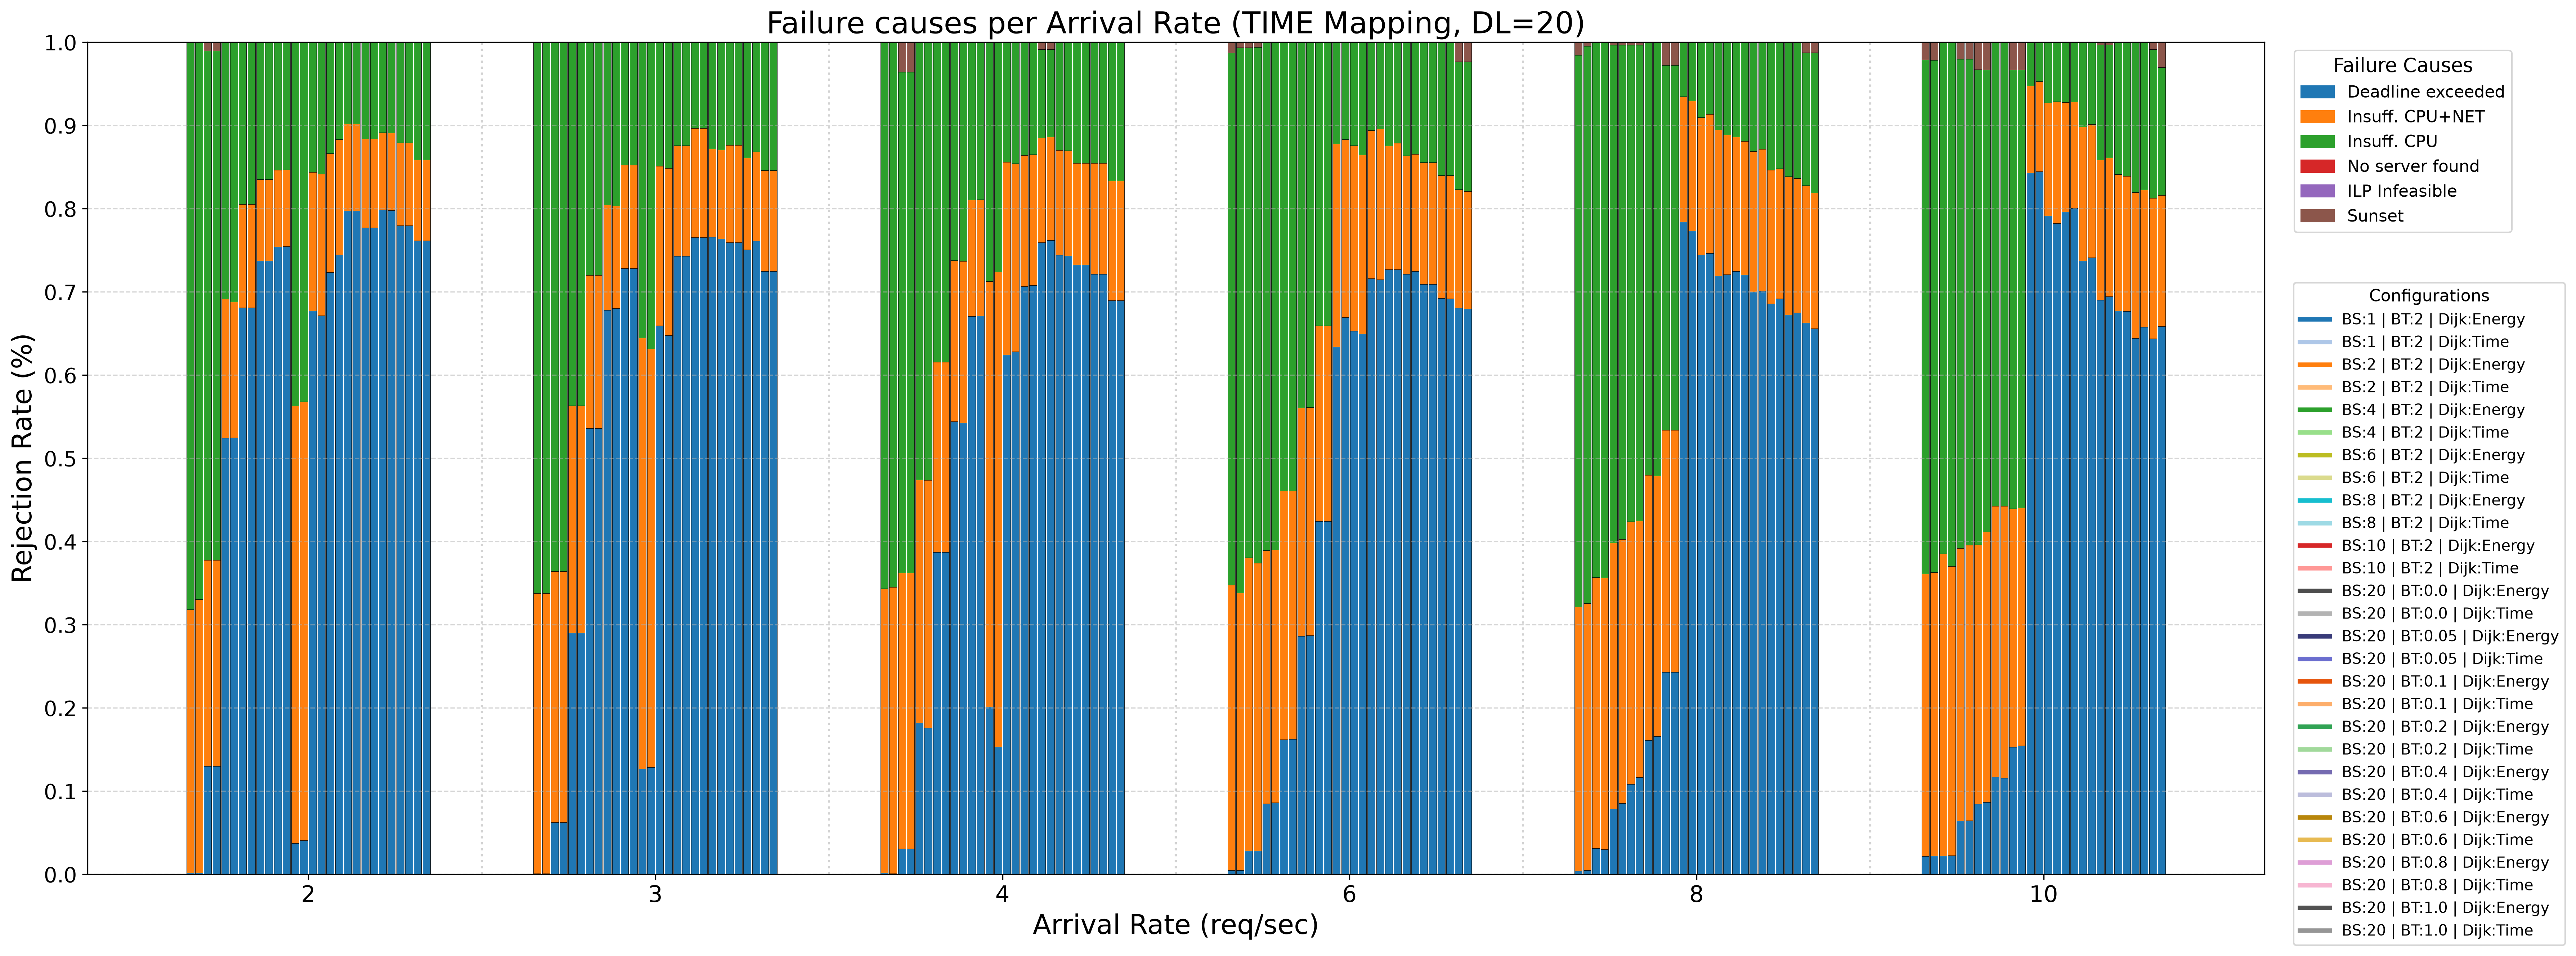
\includegraphics[width=\paperwidth]{02_Failure_Causes_time_mapping_dl_20.png}}
\captionof{figure}{Failure Causes breakdown across arrival rates ($\Delta D = 20\%$).}
\vspace{0.4em}

\makebox[\textwidth][c]{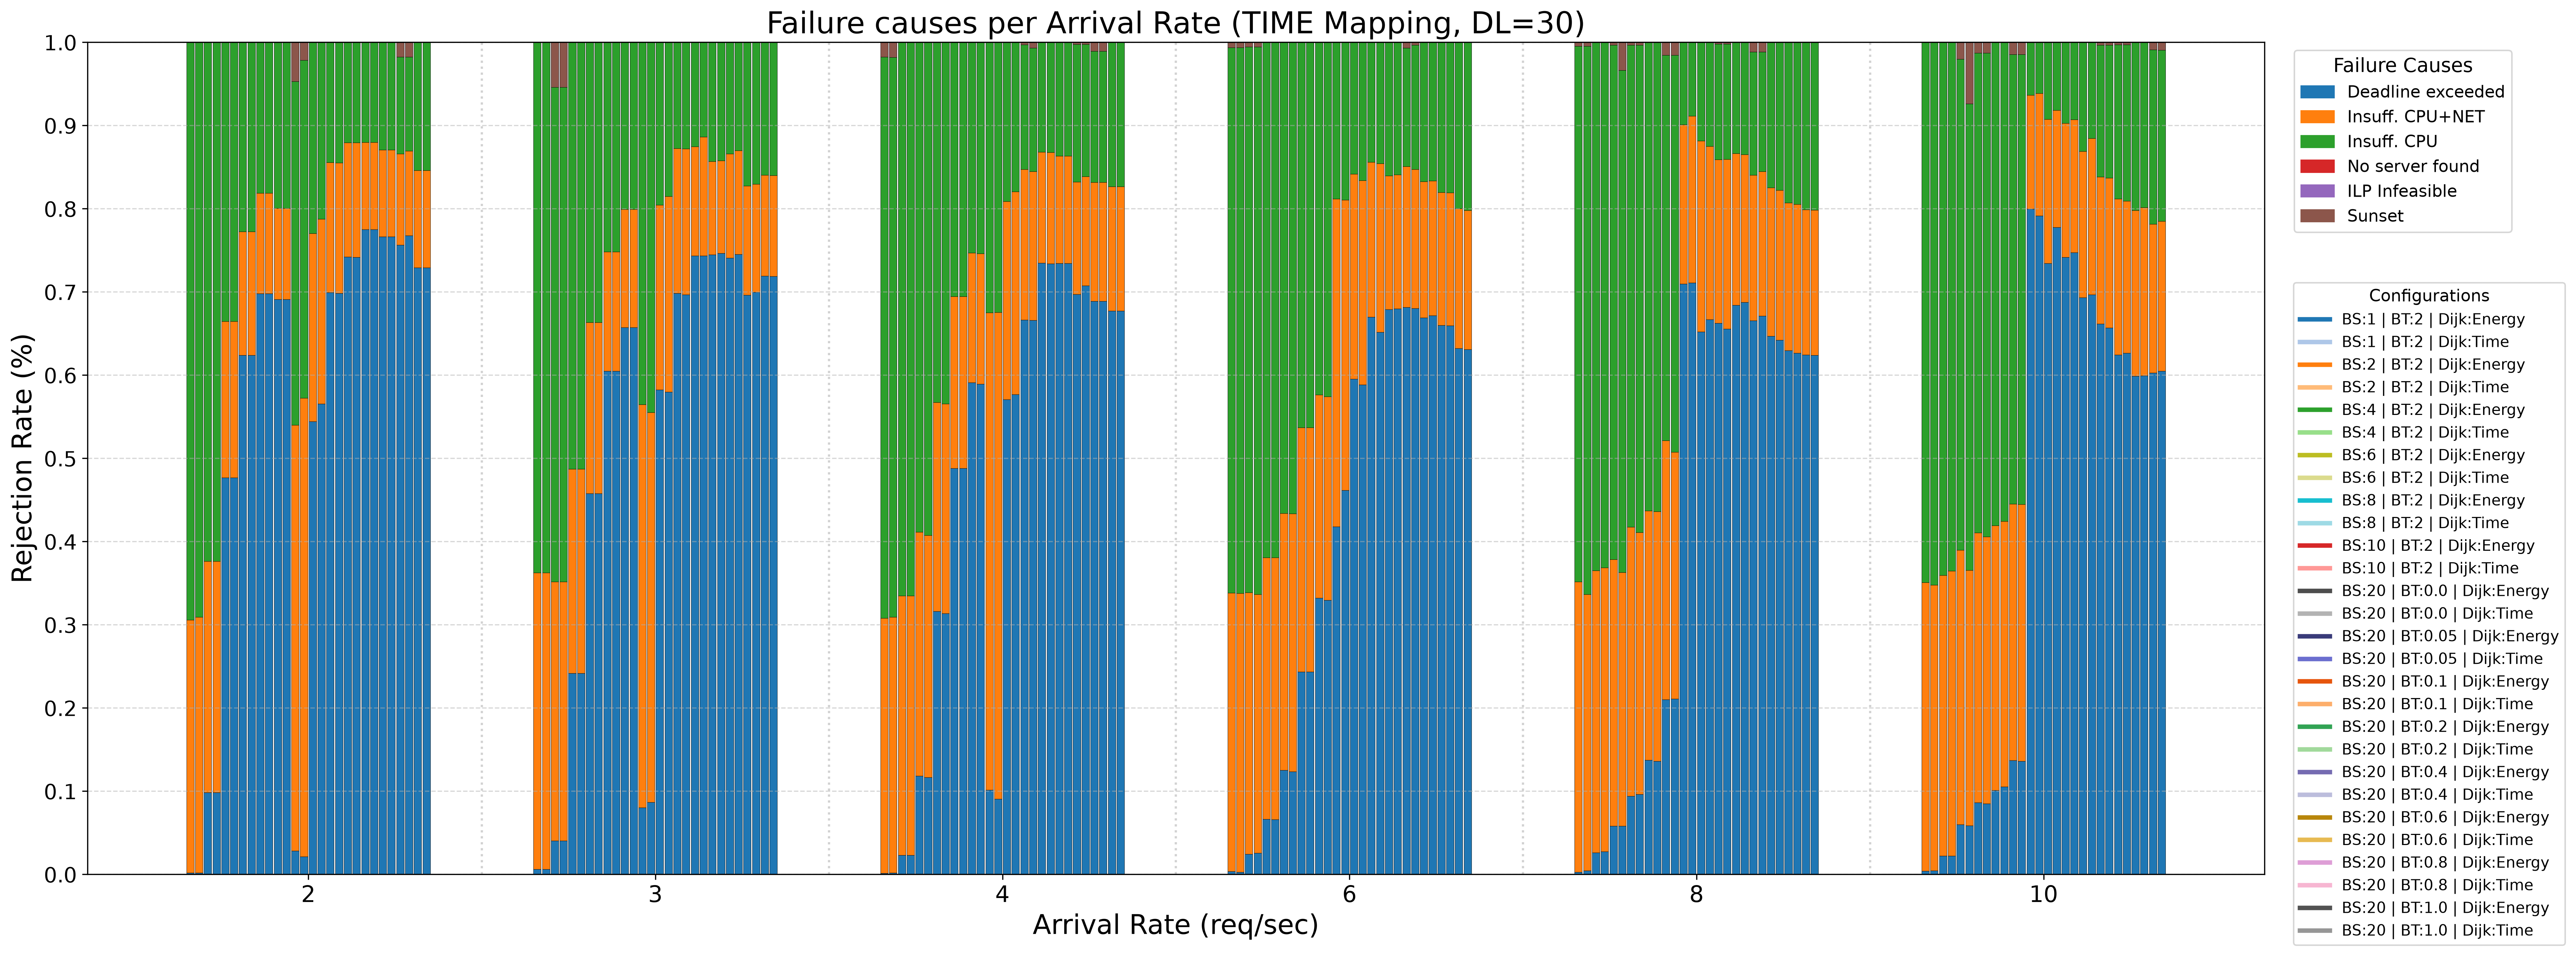
\includegraphics[width=\paperwidth]{02_Failure_Causes_time_mapping_dl_30.png}}
\captionof{figure}{Failure Causes breakdown across arrival rates ($\Delta D = 30\%$).}


La distribuzione delle cause di fallimento rivela una marcata polarizzazione architetturale: nelle configurazioni con inoltro immediato ($\text{BT} \le 0.05\text{ s}$ o $\text{BS}=1$), i rigetti sono dovuti quasi esclusivamente all'esaurimento della capacità di calcolo (\textit{Insuff. CPU}) e banda (\textit{Insuff. CPU+NET}). Al contrario, all'aumentare del timeout di batching ($\text{BT} > 0.1\text{ s}$), l'attesa in coda divora il budget temporale dei task, rendendo la violazione di scadenza (\textit{Deadline Exceeded}) responsabile del 70--85\% delle reiezioni totali. L'incremento del carico $\lambda$ intensifica progressivamente la saturazione fisica dei nodi.
\vspace{0.8em}

\clearpage

% ==============================================================================
% 3. STACKED RESPONSE TIME
% ==============================================================================

% --- Response Time: Energy Mapping (DL 10, 20, 30) ---
\begin{center}
    \textbf{\Large Stacked Response Time Breakdown --- Energy Mapping ($w_{lat}=0, w_{en}=1$)}
\end{center}
\vspace{-0.3em}

\makebox[\textwidth][c]{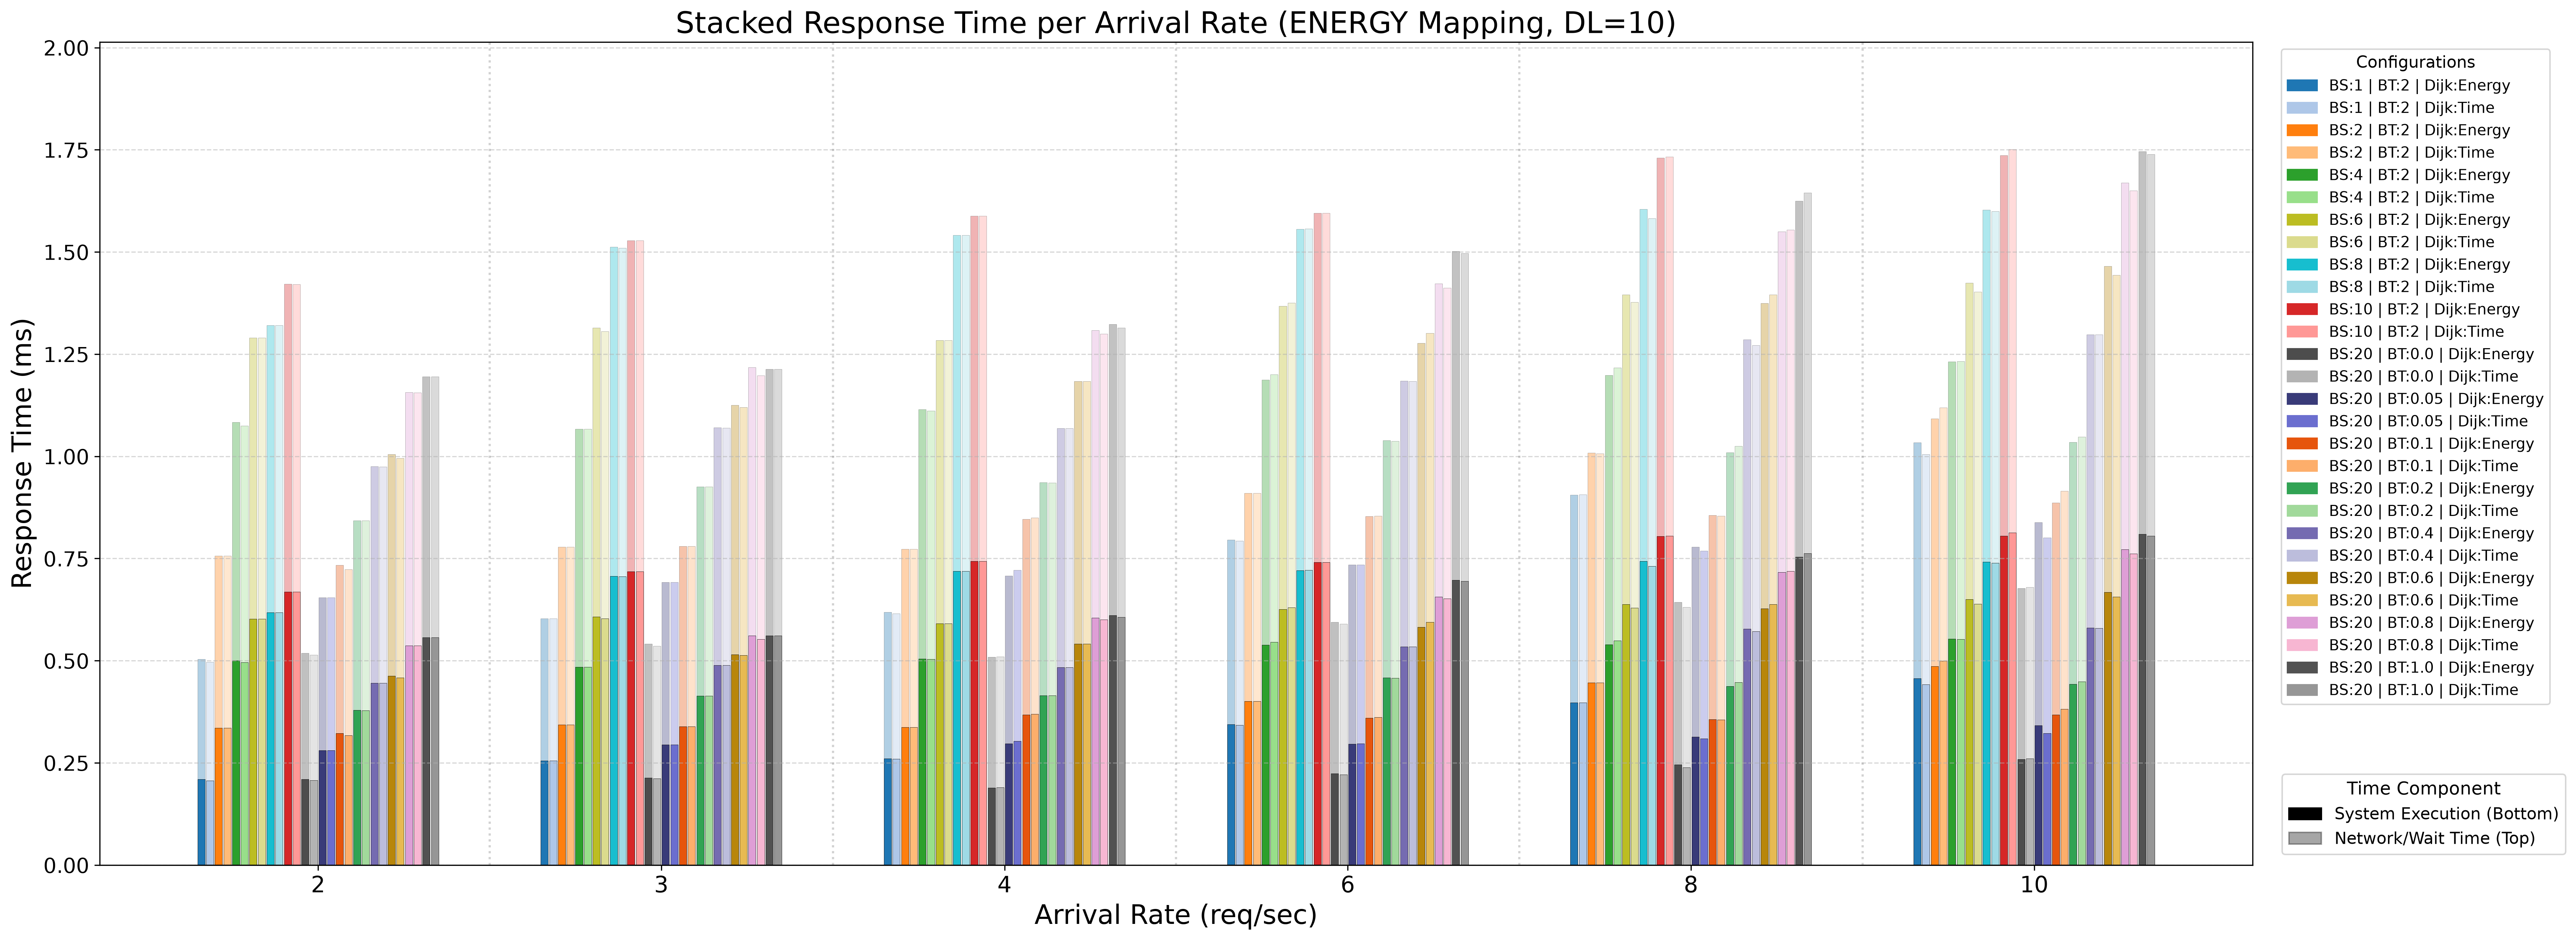
\includegraphics[width=\paperwidth]{03_Response_Time_energy_mapping_dl_10.png}}
\captionof{figure}{Stacked Response Time across arrival rates ($\Delta D = 10\%$).}
\vspace{0.4em}

\makebox[\textwidth][c]{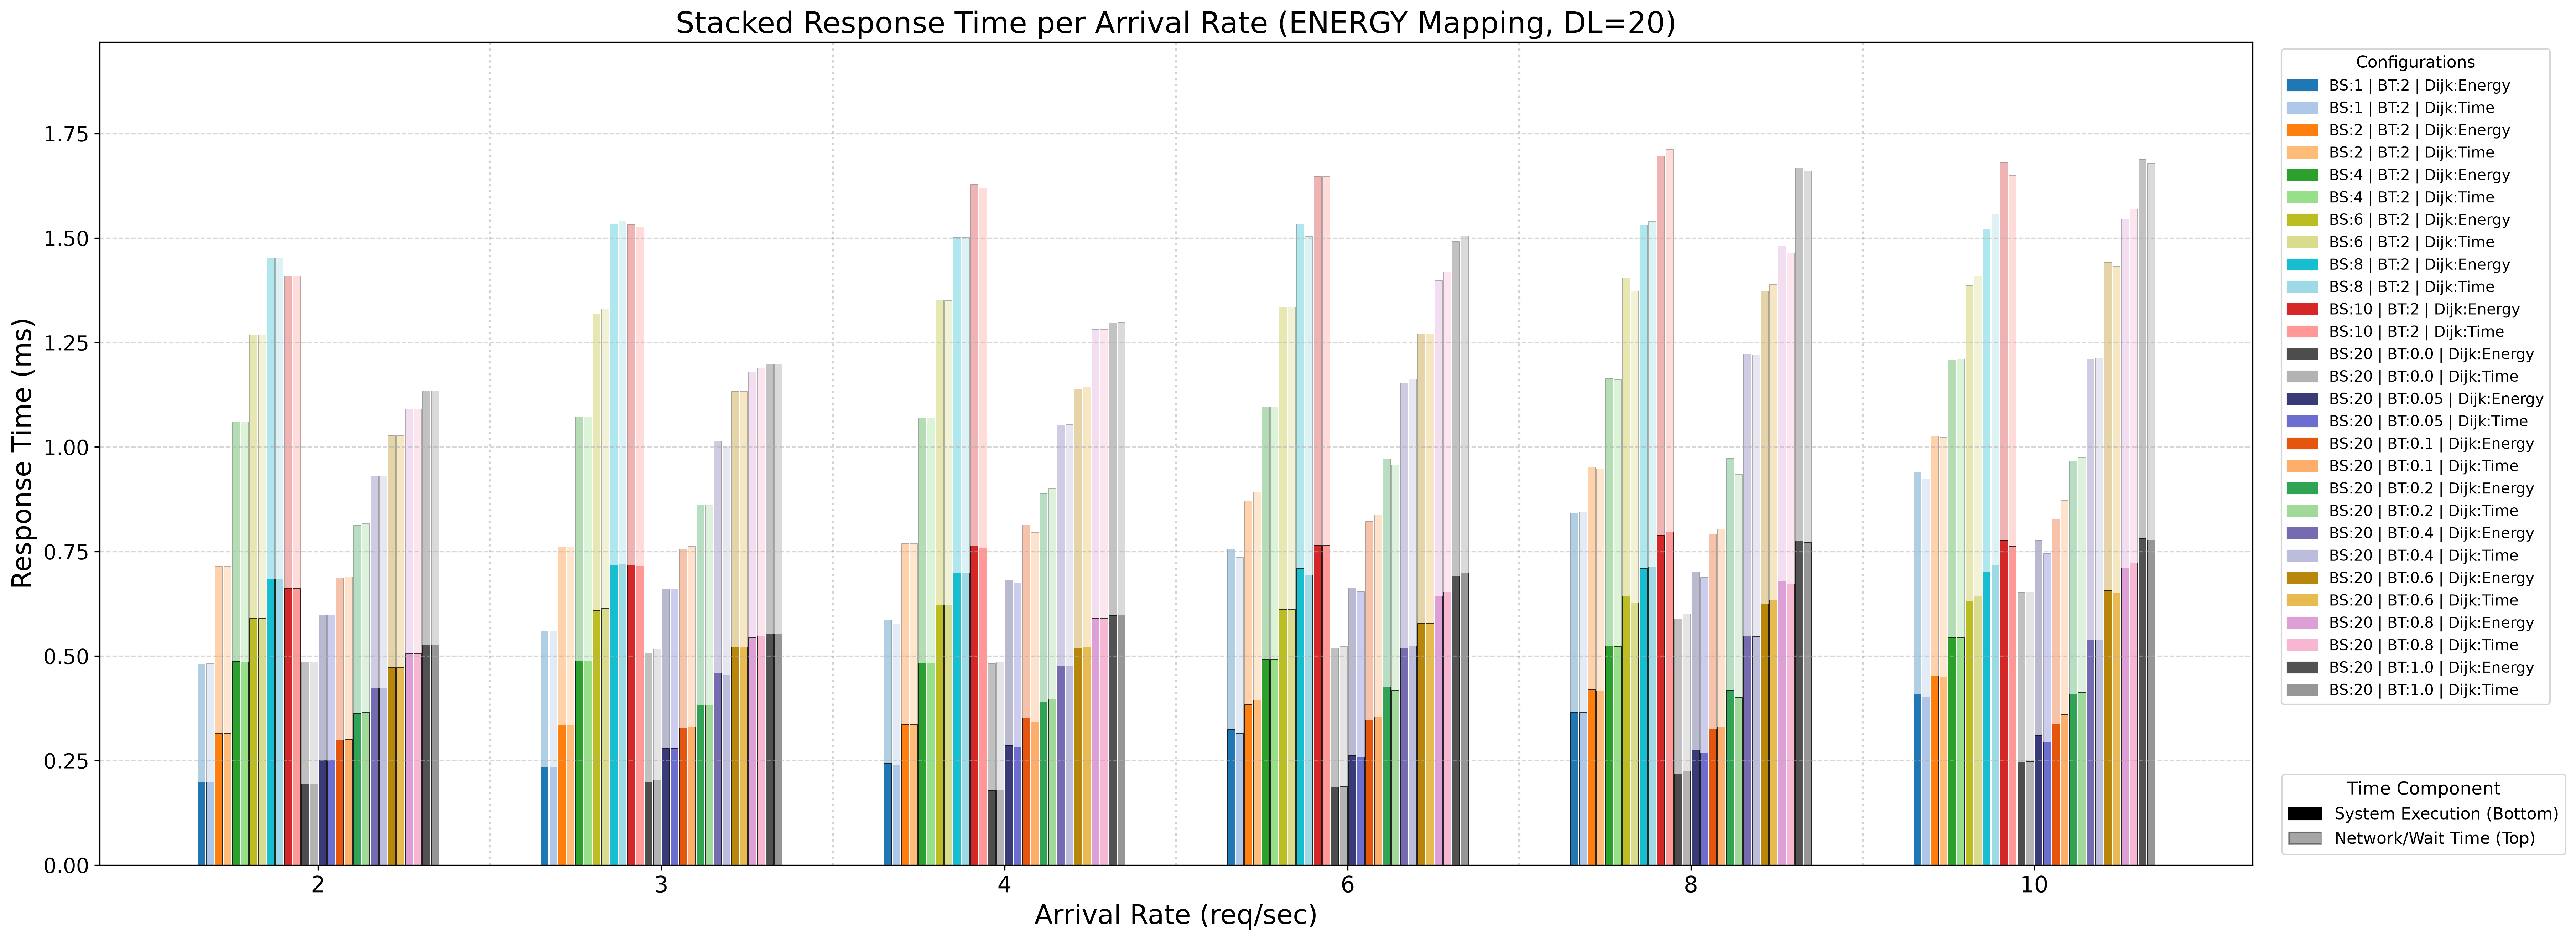
\includegraphics[width=\paperwidth]{03_Response_Time_energy_mapping_dl_20.png}}
\captionof{figure}{Stacked Response Time across arrival rates ($\Delta D = 20\%$).}
\vspace{0.4em}

\makebox[\textwidth][c]{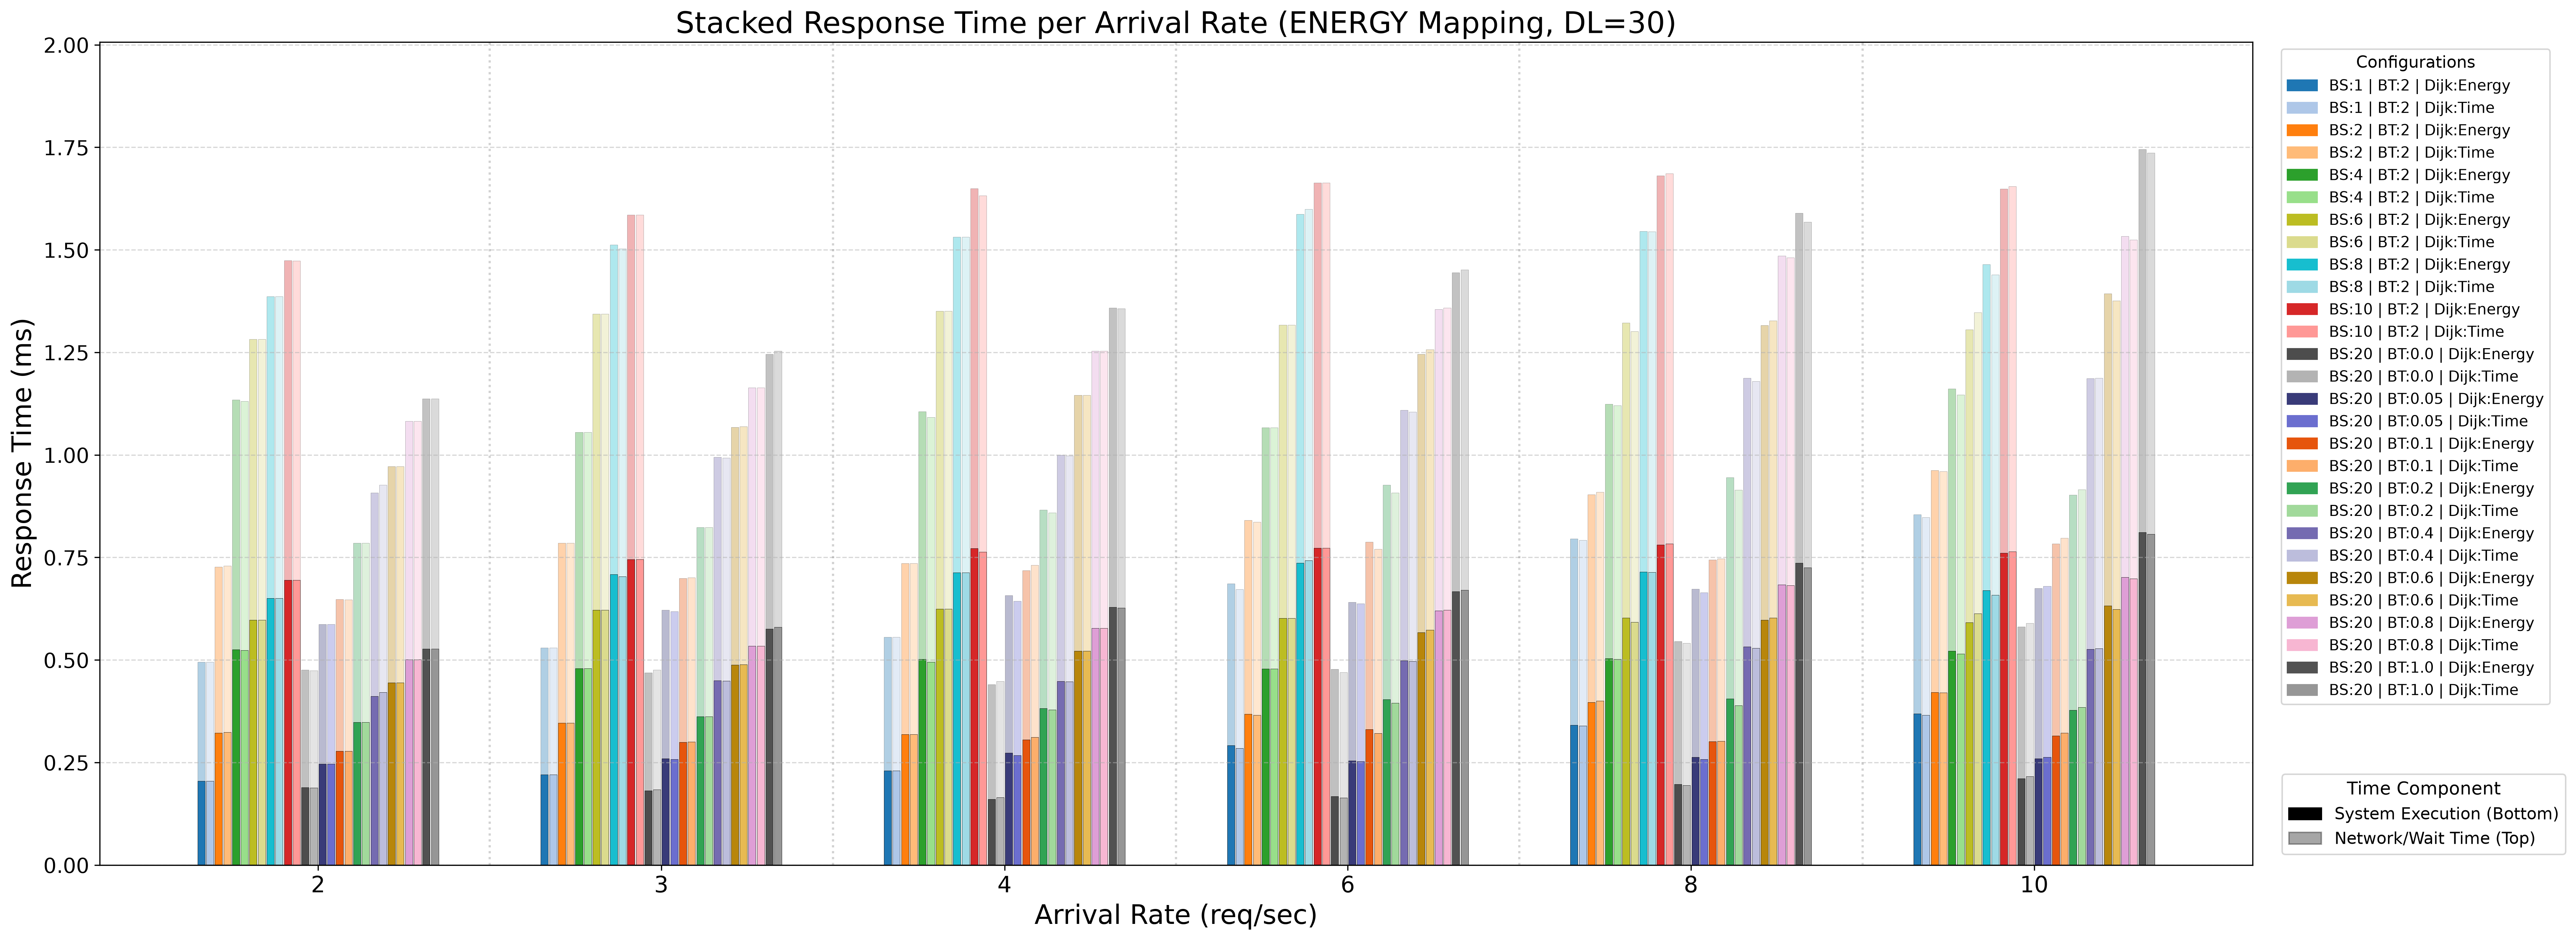
\includegraphics[width=\paperwidth]{03_Response_Time_energy_mapping_dl_30.png}}
\captionof{figure}{Stacked Response Time across arrival rates ($\Delta D = 30\%$).}



% --- Response Time: Time Mapping (DL 10, 20, 30) ---
\begin{center}
    \textbf{\Large Stacked Response Time Breakdown --- Time Mapping ($w_{lat}=1, w_{en}=0$)}
\end{center}
\vspace{-0.3em}

\makebox[\textwidth][c]{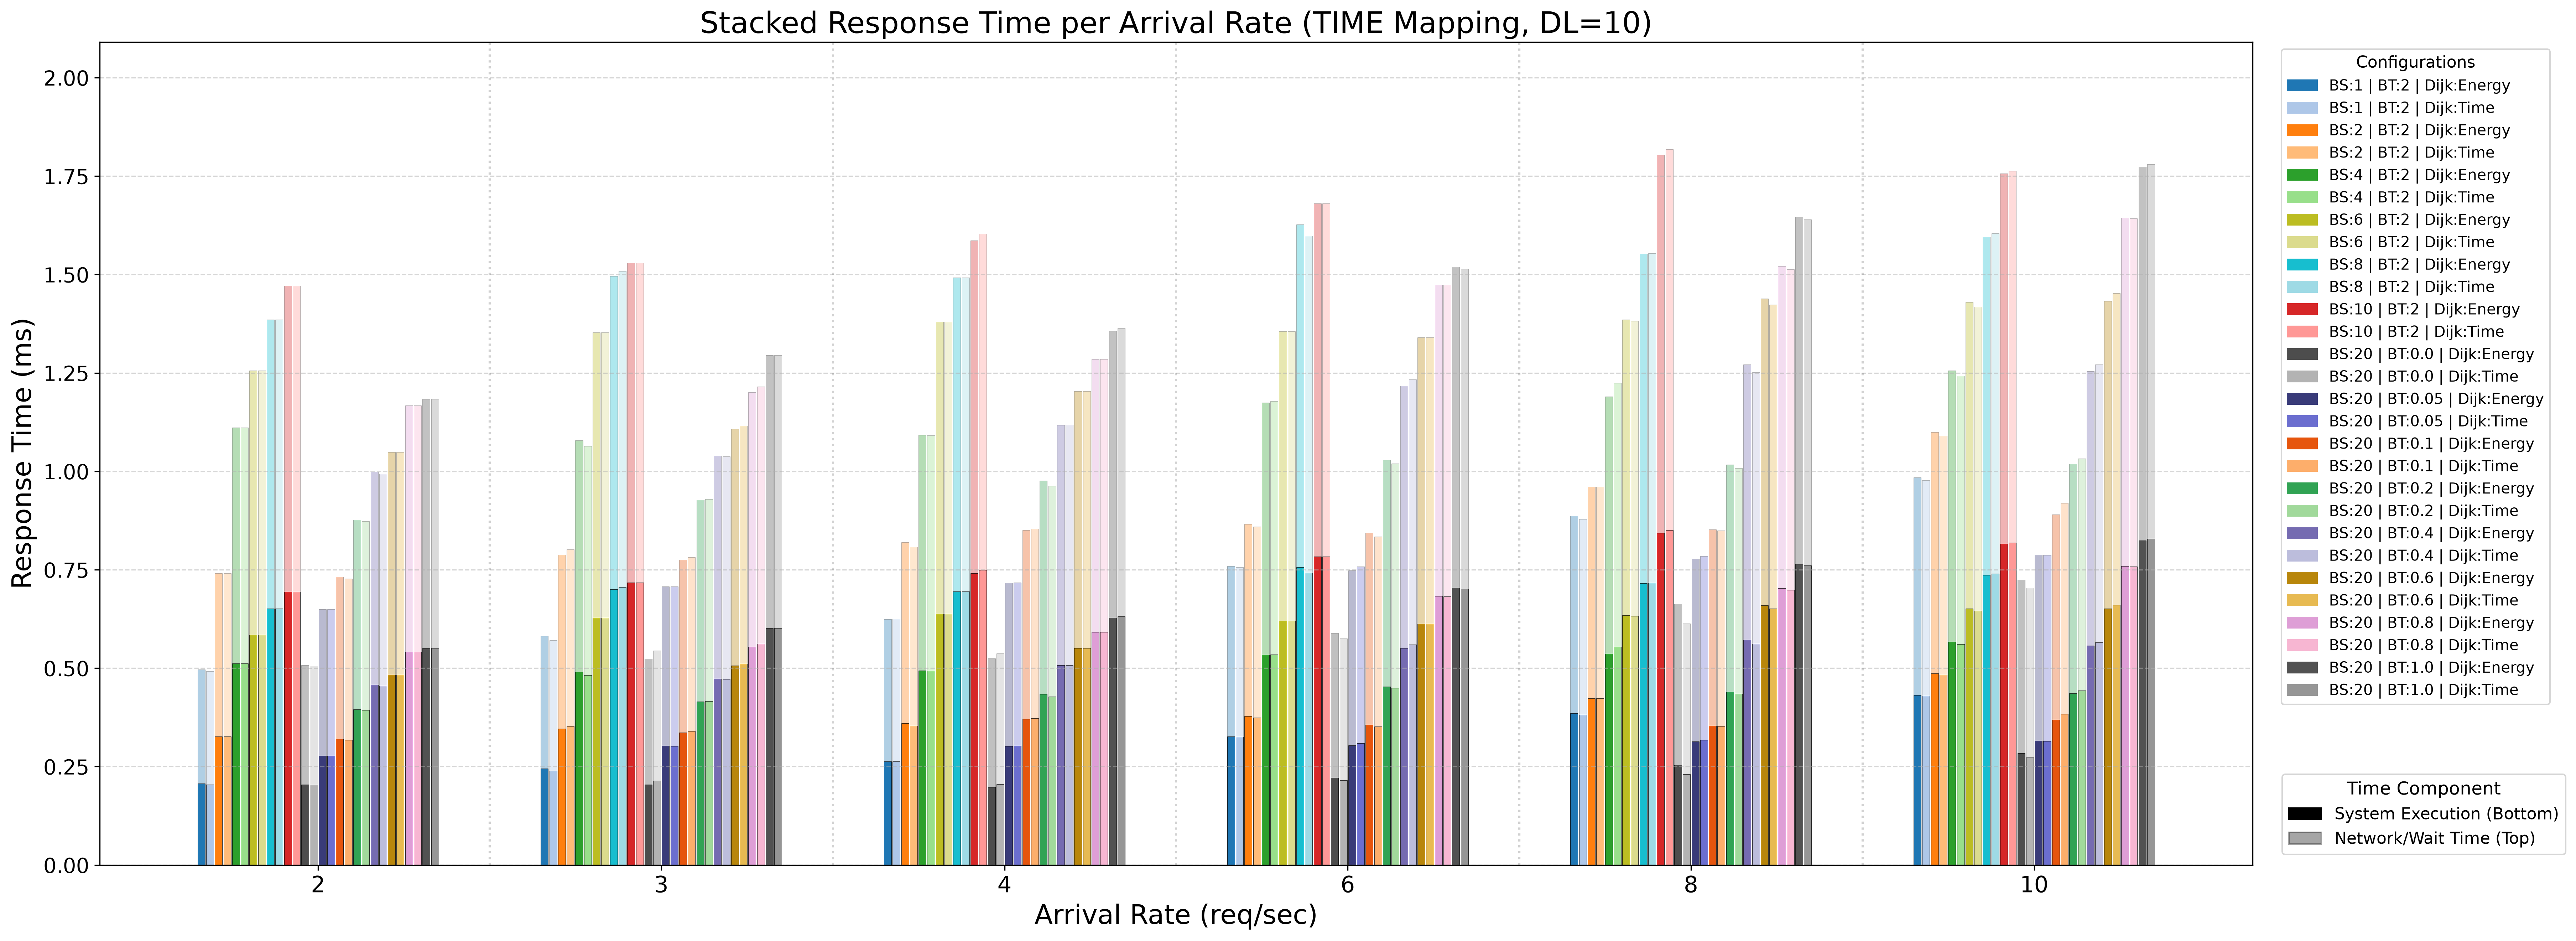
\includegraphics[width=\paperwidth]{03_Response_Time_time_mapping_dl_10.png}}
\captionof{figure}{Stacked Response Time across arrival rates ($\Delta D = 10\%$).}
\vspace{0.4em}

\makebox[\textwidth][c]{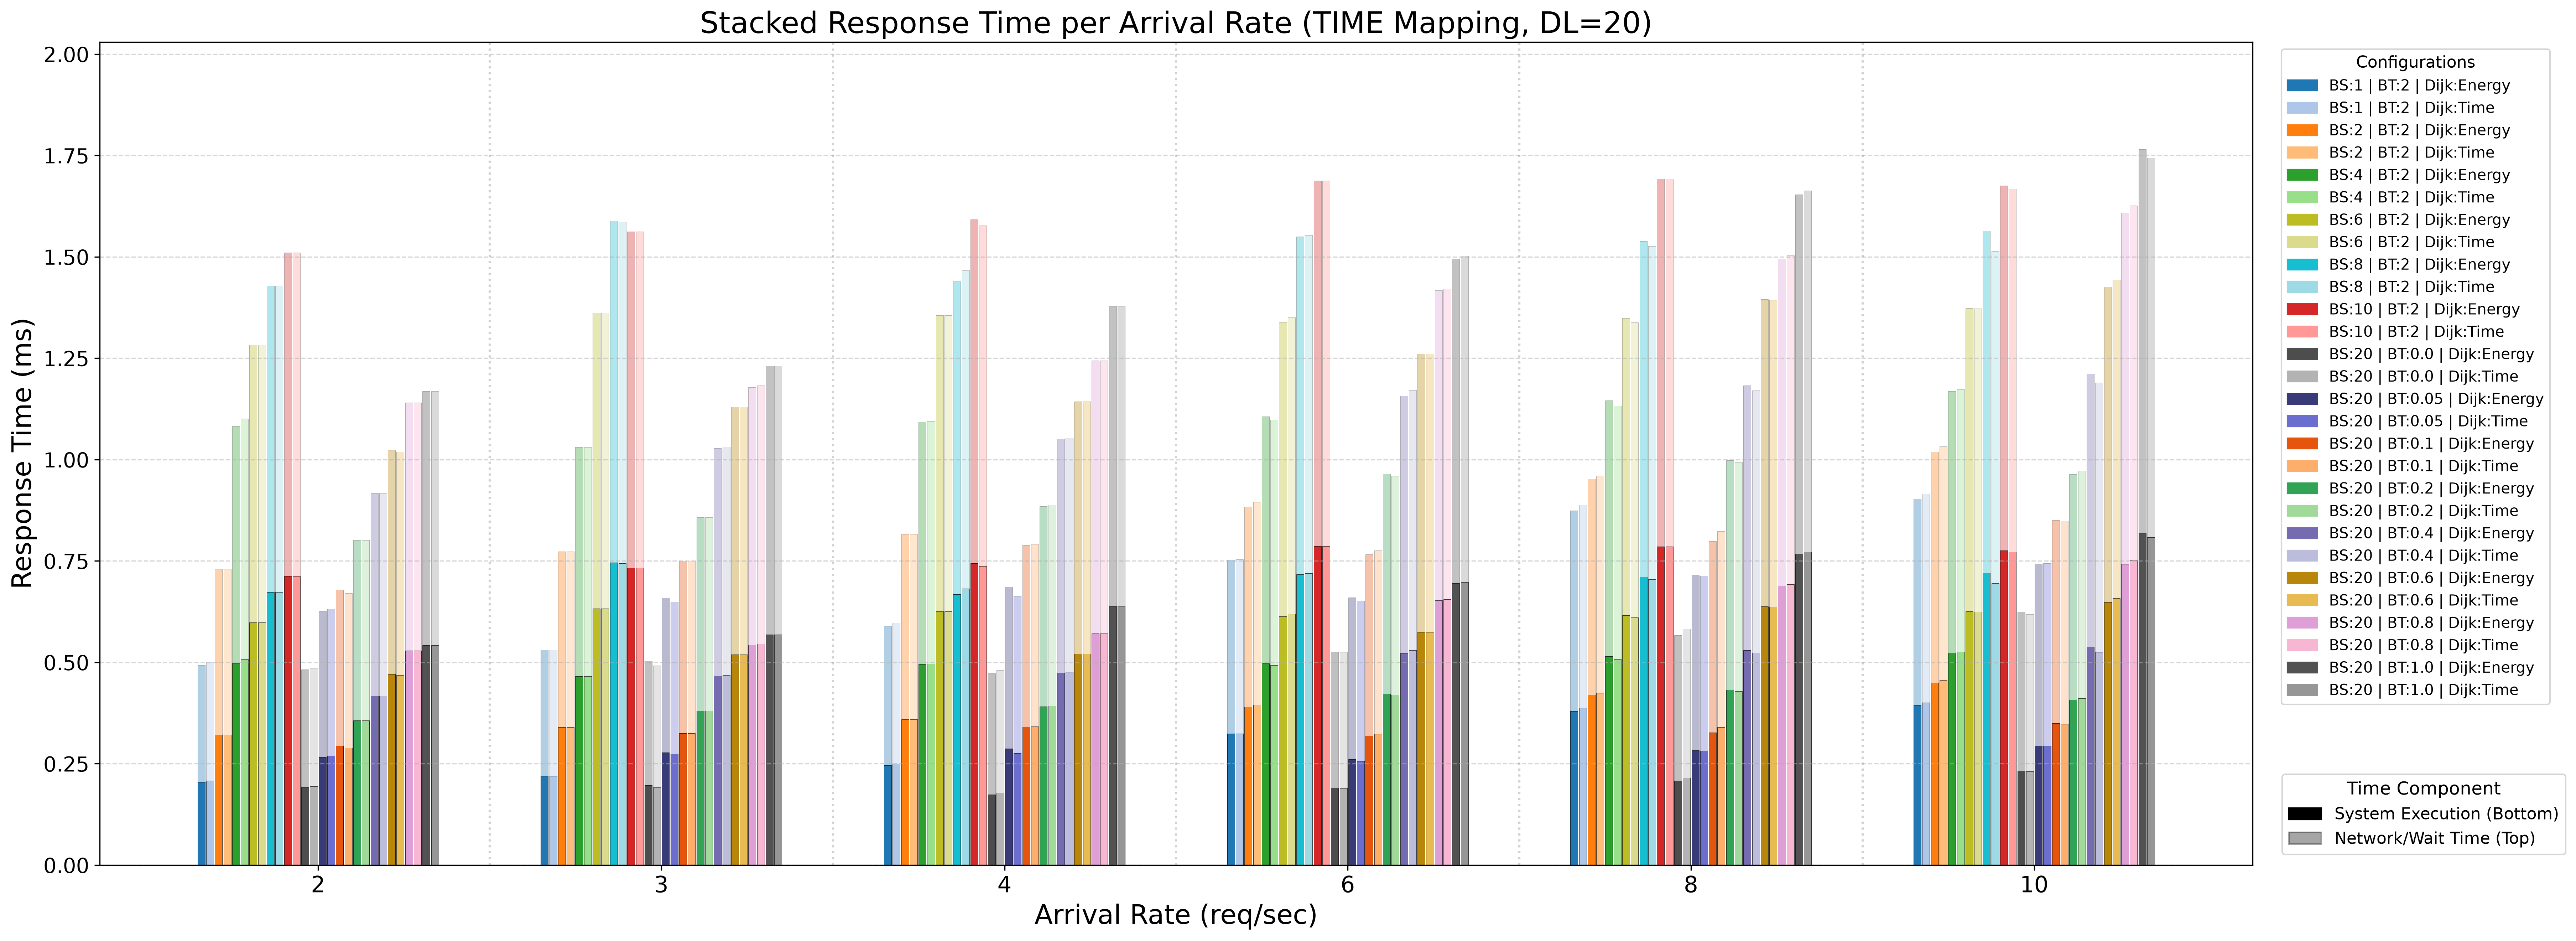
\includegraphics[width=\paperwidth]{03_Response_Time_time_mapping_dl_20.png}}
\captionof{figure}{Stacked Response Time across arrival rates ($\Delta D = 20\%$).}
\vspace{0.4em}

\makebox[\textwidth][c]{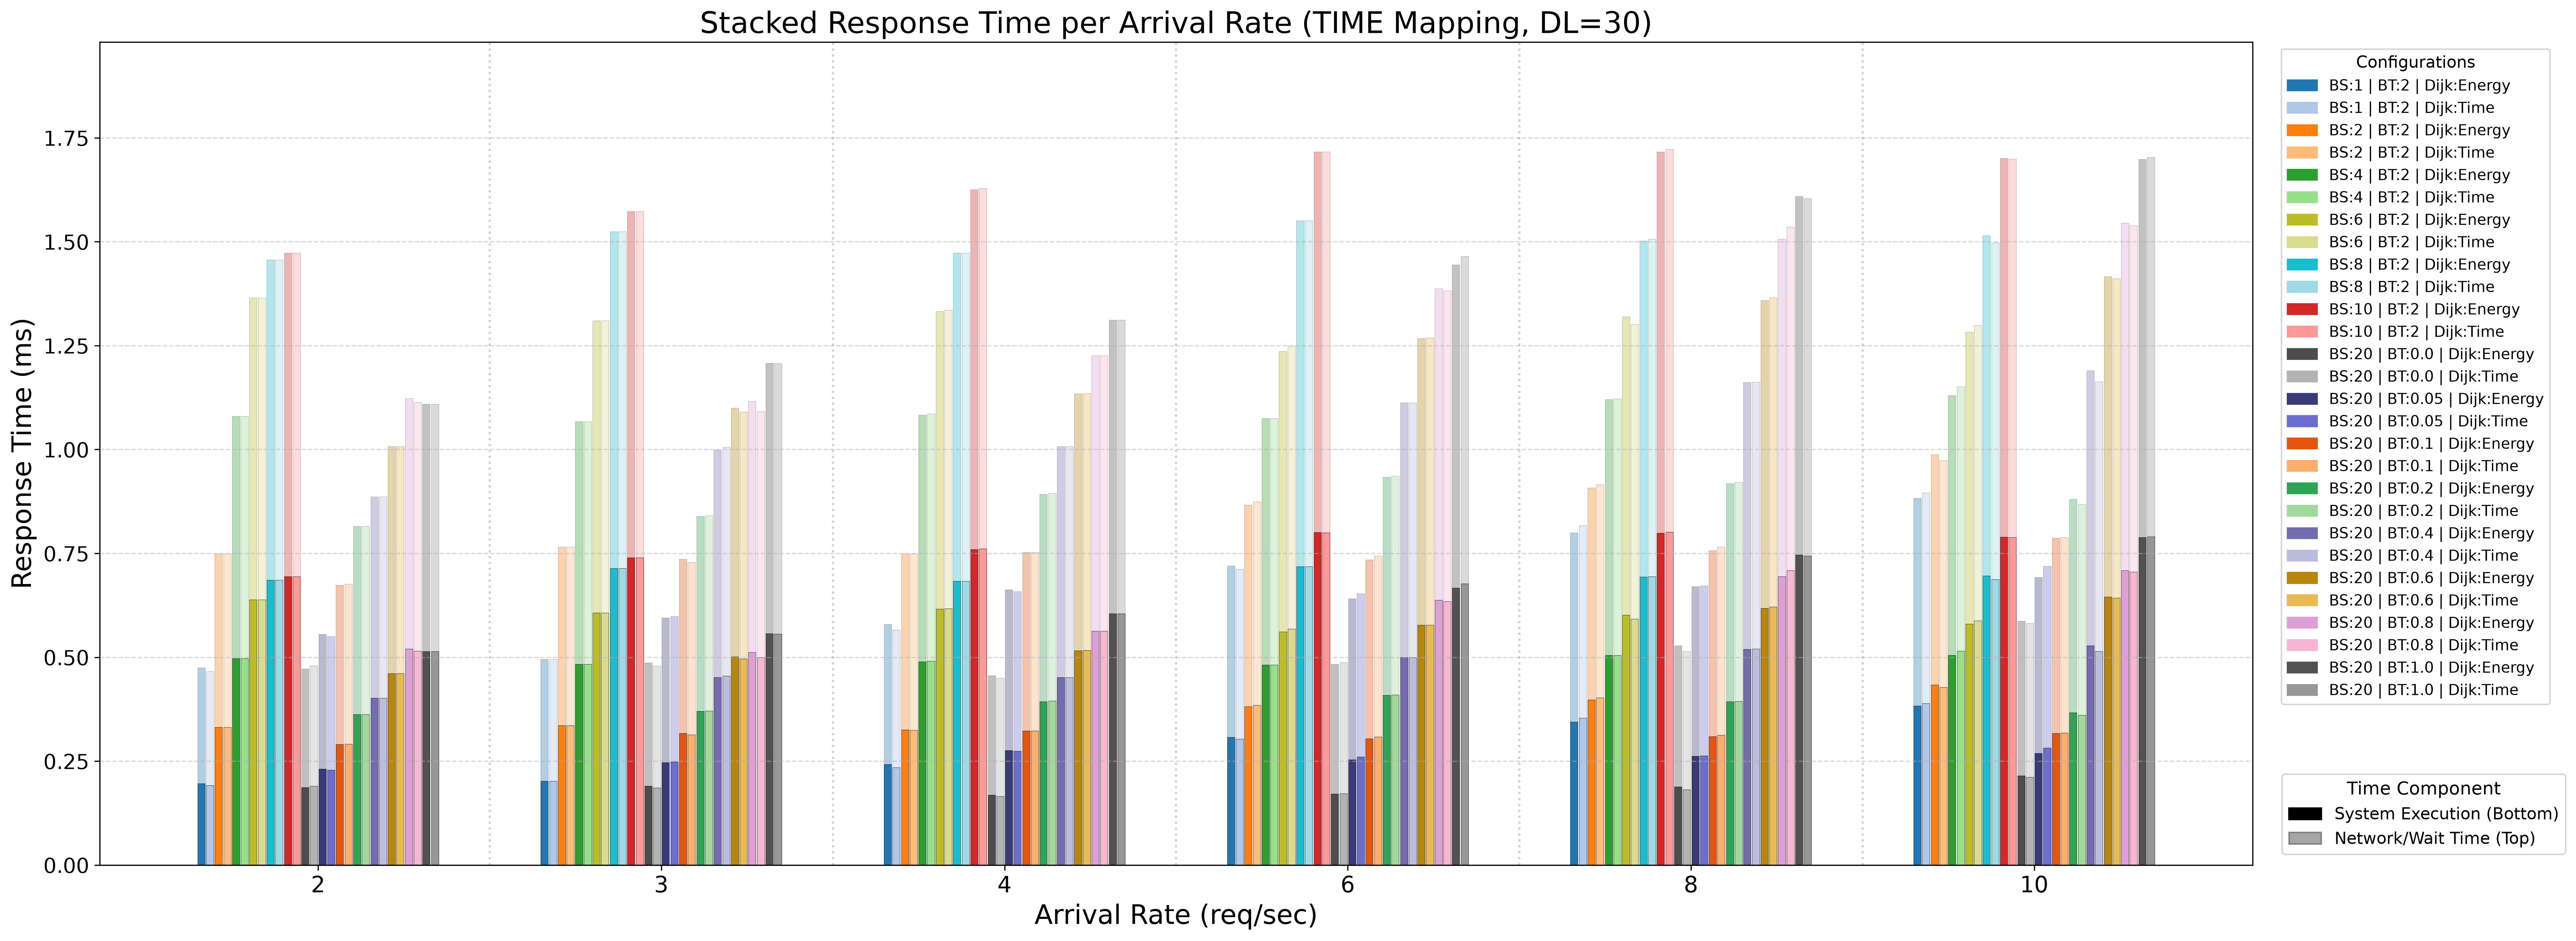
\includegraphics[width=\paperwidth]{03_Response_Time_time_mapping_dl_30.png}}
\captionof{figure}{Stacked Response Time across arrival rates ($\Delta D = 30\%$).}


La scomposizione del tempo di risposta mostra chiaramente come il tempo di calcolo effettivo del sistema (\textit{System Execution}, porzione solida inferiore) si mantenga ridotto e pressoché invariato ($\approx 0.2$--$0.7\text{ ms}$) attraverso tutte le configurazioni. La latenza end-to-end è interamente dominata dalla componente di accodamento e rete (\textit{Network/Wait Time}, porzione trasparente superiore), la quale scala in modo proporzionale a $\text{BT}$ e ad $\lambda$. Il \textit{Time Mapping} apporta solo una lievissima contrazione della latenza di rete rispetto all'\textit{Energy Mapping}, confermando che il disaccoppiamento temporale introdotto dal batching sovrasta la funzione obiettivo del solutore.
\vspace{0.8em}

\end{document}